\chapter{The Standard Model and beyond}
\label{ch:theory}

%
\begin{minipage}{\textwidth}
  {\it ``Before beginning a Hunt, it is wise to ask someone what you are looking for before you
  begin looking for it.''}

  {\hfill Winnie the Pooh, A.A.~Milne}
\end{minipage}

\vspace{2em}

This thesis contains the work undertaken in three analyses; each of which concerns a different area
of interest in \gls{HEP}.
The following chapter aims to motivate each analysis in turn after introducing the Standard Model
of particle physics.

Firstly, the formulation of the \sm will be outlined, with particular detail paid to the flavour
sector.
Various successes of the \sm will then be discussed before going on to identify its shortcomings
using arguments from both experiment and theory.
These shortcomings will then be used to motivate the three analyses:
a search for the decay \btodsphi (\Chap{ch:dsphi});
a search for the two related decays \btokpipimumu and \btophikmumu (\Chap{ch:hhh});
a search for dark sector particles in $\decay{\Bd}{K^*(892)^0}$ (\Chap{ch:db}).
Theory specific to each of these analyses will be detailed in the relevant chapter.

%The convension of natural units, $c=\hbar=1$, is assumed throughout.
%Indices for four vectors are labelled by $\mu$ and $\nu$, and indices for the $SU_C(3)$ and
%$SU_L(2)$ generators are

%The following chapter will elucidate as to how the flavour sector is the only source of \CPV in the
%SM.
%It will then go on to motivate study of flavour physics at \lhcb by exploring some problems with
%the SM as a theory.

%\section{The Standard Model}
The current formulation of the SM of particle physics was concocted in the 1970s, when the Higgs
mechanism was incorporated into Glashow's electroweak theory by Salam and Weinberg.
The theory prescribes a treatment
as to how fundamental particles interact via three of the four
fundamental forces, namely: the strong, weak and electromagnetic forces.

%Mathematically, the SM is a locally gauge invariant quantum field theory, where excitations of
%various fields manifest themselves as particles.
%There is a global Poincare symmetry as required by special relativity; and a local
%$SU(3)\times SU(2)\times U(1)$ symmetry which encapsulates the SM Lagrangian:
%\begin{equation}
  %\Lag{SM} = \Lag{EW} + \Lag{Strong} + \Lag{Higgs}.
%\end{equation}
%Where the components describe the electroweak, strong and Higgs interactions.
%Each generator of this local gauge group is associated with a gauge boson which mediates
%interactions between other bosons and fermions.

Mathematically, the SM is a locally gauge invariant quantum field theory.
It inhabits a space-time with a global Poincar\'e symmetry that obeys a local
$SU(3)\times SU(2)\times U(1)$ symmetry.
Each generator in this group corresponds to a gauge-boson; so the strong force ($SU(3)$ group) has
eight gluons that mediate the interaction, and the electroweak force ($SU(2)\times U(1)$ group) has
$3+1$ gauge bosons, which are the weak gauge bosons ($Z$, $W^\pm$) and the photon ($\gamma$).
These are all vector fields.
Fermions are described by spinor fields, $\psi$, which obey the Dirac equation:
\begin{equation}
  (i\hbar\gamma^\mu\partial_\mu - mc)\psi = 0.
  \label{th:eq:dirac}
\end{equation}
The fermions of the SM constitute six leptons (electron, electron neutrino, muon, muon neutrino,
tau and tau neutrino) and six quarks (up, down, charm, strange, top and bottom), which are
organized into pairs forming three generations.
For each fermion there is a corresponding antiparticle with the same mass and opposite charge ---
charge being the conserved quantity resulting from the global gauge symmetry (by Noether's
theorem).
There is also a single scalar field in the SM, that of the Higgs boson.
%The only additional particle is the scalar Higgs boson.

The SM Lagrangian can be expressed as a sum of components:
\begin{equation}
  \Lag{SM} = \Lag{QCD} + \Lag{V} + \Lag{\ell} + \Lag{\it q} + \Lag{Higgs} + \Lag{Yuk}.
  \label{eq:th:lag}
\end{equation}
The first term describes interactions of the strong force between colour carrying particles in the
theory of Quantum Chromodynamics (QCD).
Descriptions of weak vector boson self-interactions, and the electroweak behavior of
leptons are encapsulated in the next two terms.
Finally, the remaining terms describe the electroweak behavior of quarks, the Higgs interaction and Yukawa
couplings, respectively.
These latter terms are of fundamental importance as to how flavour changing currents and CPV
occur in the SM. %, and will be be discussed in detail.
%the SM.
%Each of these shall be discussed in turn.

%\subsection{Uncertainties in theoretical predictions}
\section{Dealing with QCD}

For the branching fractions discussed in this thesis, theoretical uncertainties from \QCD make
predictions difficult\footnote{
  The following section is based on Refs.~\cite{Pich:1998xt}.
}.
Quantum Chromodynamics describes the interactions of colour charged particles (quarks and
gluons).
%interactions between quarks via the strong force which is mediated by gluons.
The behaviour of \QCD exhibits two peculiarities: confinement, and asymptotic freedom.
Confinement describes the strong force over long distances ($\approx1\fm$)
where, unlike QED, the interaction strength does not lessen with distance.
This means that as a quark is separated from others, there is enough energy in the gluon field to
create a new quark-antiquark pair.
The resulting bound states always have net zero colour charge.
Therefore, free quarks are never observed over macroscopic distances
and are observed as mesons (quark-antiquark bound states), baryons (bound states of
three quarks), or tetra-quarks~\cite{LHCb-PAPER-2014-014}.
%but are seen to behave as free
%particles in deep inelastic scattering.
Asymptotic freedom means that forces between quarks become asymptotically weaker as the energy of
the system increases --- and the distance decreases.

Predictions of $b$-hadron processes involving \QCD can also be made using effective field theory.
Despite the large mass of the \bquark quark with respect to $\Lambda_\mathrm{QCD}\simeq200\mev$,
the system can be treated perturbatively since $\alpha_\mathrm{QCD}(m_\bquark)$ is sufficiently
small.
This is known as a Heavy Quark Effective Theory (HQET).
In contrast to an EFT where the weak fields have been integrated out, in a HQET
it is not possible to remove heavy quark contributions entirely because the \bquark quark
cannot decay without violating flavour number.
This essentially treats a $b$-hadron like a hydrogen atom, where the \bquark quark takes
the place of the nucleus, allowing for a highly simplified theoretical treatment, with corrections
of order $m_\bquark^{-1}$.

Despite the use of HQET, the fact is that hadrons are inherently non-perturbative objects, and so
it is useful to make further assumptions.
An important supposition is that of \emph{factorization} which assumes that the short-distance,
process dependent, \QCD effects are separable from hadronization, the long distance effects.
Hadronization is very difficult to calculate with \QCD, for this reason form-factors are used to
empirically encapsulate the process.
Form-factors must be measured experimentally and are the dominant source of uncertainty in the
calculation of $B$ mesons decaying into hadronic (or semi-hadronic) final states.





%The mass of the \bquark quark is sufficiently high that QCD calculations in $B$ decays can be made
%using peturbation theory.
%Furthermore, initial conditions can modelled using Heavy Quark Effective Theory (HQET), which
%essentially models a bound state of a heavy and light quark like a hydrogen atom, with the \bquark
%taking the role of the nucleus.
%However, this latter approximation breaks down at low energies where the hadron has an energy
%comparable to the mass of the \bquark quark.

%Another important assumption for QCD predictions is that of factorizability.
%A decay is factorizable if one can separate the initial, partonic, state from the hadronization of
%the final state quarks.
%Hadronization is very difficult to model, and therefore empirical models, encoded into
%form-factors, are used.
%It is these form-factors which are the dominant source of theoretical uncertainty.


%These oddities mean that QCD must be dealt with in different ways depending on the energy regime of
%interest.
%For high momentum interations the coupling strength, $\alpha_\mathrm{QCD}$ is small and the system
%can be dealt with using peturbation theory.
%But, for low momentum interactions $\alpha_\mathrm{QCD}$ increases because of the
%\emph{running} of the coupling.
%In the latter regime the system cannot be modelled with peturbation theory because it is not
%infrared safe and rather Lattice QCD must be used.
%Another inadequacy of peturbation theory is that it considers asymptotic states of quarks and
%gluons as free states, where in actuallity the physical states which are observed are hadrons.
%
%Difficulties with calculating QCD interactions leads to the necessity of form factors, which are
%empirical functions with parameters measured experimentally.
%These are
%
%
%\begin{itemize}
  %\item Heavy quark effective field theory simpolify calculations
    %interactions of the heacy wuark are soft cmopared tot the large mass of the $B$, and partonic
    %process is expanded in terms of $\Lambda_{QCD}/m_B$
  %\item QCD factorization setarates partonic process from the hadronisation of the $sq$ pair
  %\item Hadronisation is encoded into hadronic form-factors which is the dominant source of
    %uncertainty for theoretical predictions
%\end{itemize}








%The following chapter will elucidate as to how the flavour sector is the only source of CPV in the
%SM.
The structure of CP and flavour violation emerges as a direct consequence of the Higgs mechanism
breaking the local electroweak symmetry.
The Lagrangian of the scalar Higgs field is:
\begin{align}
  \Lag{Higgs}
  &= \left(D_\mu\Phi\right)^\dagger\left(D^\mu\Phi\right) - V(\Phi) \\
  &= \left(D_\mu\Phi\right)^\dagger\left(D^\mu\Phi\right) - \mu^2\left(\Phi^\dagger\Phi\right) +
  \lambda\left(\Phi^\dagger\Phi\right),
  \label{eq:th:laghiggs1}
\end{align}
where $\mu$ and $\lambda$ are constants, $D_\mu$ is the covariant derivative, and $\Phi$ is the
Higgs doublet, defined by:
\begin{equation}
  \Phi = \frac{1}{\sqrt{2}}
  \begin{pmatrix}
    \phi_1 + i\phi_2 \\
    \phi_3 + i\phi_4 \\
  \end{pmatrix}.
  \label{eq:th:phi}
\end{equation}
Taking $\mu^2<0$ and $\lambda>0$ moves the minimum of the potential $V(\Phi)$ away from zero to a distance $v$:
\begin{equation}
  v = \sqrt{\frac{\mu^2}{\lambda}}.
\end{equation}
At this point the Higgs field gets a vacuum expectation value (VEV)
%$\braket{\phi} = \tfrac{1}{\sqrt{2}}v$.
of $\langle\phi\rangle = \tfrac{1}{\sqrt{2}}v$.
The direction of the VEV from the origin is arbitrary, but the choice of:
\begin{align}
  \bra{0}\phi_1\ket{0} =
  \bra{0}\phi_2\ket{0} =
  \bra{0}\phi_4\ket{0} = 0  &&
  \bra{0}\phi_3\ket{0} = v,
\end{align}
is convenient, and changes Eq.~\ref{eq:th:phi} to:
\begin{equation}
  \Phi = \frac{1}{\sqrt{2}}
  \begin{pmatrix}
    \eta_1 + i\eta_2 \\
    v + i\eta_4 \\
  \end{pmatrix}.
  \label{eq:th:eta}
\end{equation}
Here, $\eta_1$, $\eta_2$ and $\eta_4$, are Goldstone bosons which, by choosing an appropriate
gauge, become the longitudinal components of the weak bosons.
This choice of gauge simplifies $\Phi$ to:
\begin{equation}
  \Phi =
  \begin{pmatrix} 0 \\ v+H
  \end{pmatrix},
  \label{eq:th:phi2}
\end{equation}
where $H$ is the physical Higgs boson.
%Using this in Eq.~\ref{eq:th:laghiggs1} gives:
Inserting Eq.~\ref{eq:th:phi2} into Eq.~\ref{eq:th:laghiggs1} gives:
%\begin{multline}
  %\Lag{Higgs} =
  %\frac12\left(\partial_\mu H\right)\left(\partial^\mu H\right)
  %+\frac14g^2\left(v^2 + 2vH + H^2\right)W_\mu^+W^{-\mu}  \\
  %+\frac18\left(g^2 + g^{\prime2}\right)\left(v^2 + 2vH + H^2\right)Z_\mu Z^\mu
  %+ \mu^2H^2 + \frac14\lambda\left(H^4+4vH^3\right) + \cdots,
  %\label{eq:th:laghiggs2}
%\end{multline}
\begin{equation}
  \Lag{Higgs} =
  \frac12\left(\partial_\mu H\right)\left(\partial^\mu H\right)
  +\mu^2H^2
  +\left(m_W^2W_\mu^+W^{-\mu} + \frac{m_Z^2}{2}Z_\mu Z^\mu\right)
  \cdot
  \left(1 + \frac{H}{v}\right)^2
  \label{eq:th:laghiggs2}
\end{equation}
where $g$ and $g^\prime$ are coupling constants and other terms are three- and four-point
interactions of the Higgs with itself and weak gauge bosons.
Thus, the $U(1)$ local gauge symmetry is broken, weak gauge boson acquire a mass while photons remain
massless; as is consistent with observations.


%It is not possible to directly insert mass terms for fermions, because the required terms
%($m(\bar\psi_L\psi_R+\bar\psi_R\psi_L$) are not allowed \bam{ELABORATE}.
All fermions (except neutrinos) also get a mass after the spontaneous symmetry breaking (SSB) of
the $U(1)$ symmetry.
The Dirac mass term for a chiral field should be of the form:
\begin{equation}
  \Lag{mass} = -m_\psi\left(\bar\psi_R\psi_L + \bar\psi_L\psi_R\right),
\end{equation}
but the left- and right-handed fields have different $U(1)$ charges %Y hypercharge
and so transform differently under local gauge transformations and so cannot be added to \Lag{SM}.
However, masses can be generated through the Yukawa couplings (\Lag{Yuk} in \Eq{eq:th:lag}), which
describe integrations between all fermionic fields and the Higgs doublet, and can be written:
\begin{equation}
  \Lag{Yuk} = \sum_{\substack{\ell=\\e,\mu,\tau}}\left(\Lag{Yuk}^\ell\right) + \Lag{Yuk}^q,
  \label{eq:th:yukking}
\end{equation}
where $\ell$ and $q$ denote the lepton and quark sectors respectively.
First considering the lepton term, after SSB:
\begin{align}
  \Lag{Yuk}^\ell
  &= - g_\ell\left(\bar\chi_L\Phi \ell_R + \bar \ell_R\Phi^\dagger\chi_L\right) \\
  &= - \frac{g_\ell v}{\sqrt{2}}\left(\bar\ell_L\ell_R + \bar\ell_R\ell_L\right)\cdot
  \left(1 + \frac{H}{v}\right)
     %- \frac{g_\ell}{\sqrt{2}}H\left(\bar\ell_L\ell_R + \bar\ell_R\ell_L\right),
\end{align}
where $g_\ell$ is a coupling constant, and
\begin{align}
  \chi_L = \begin{pmatrix}\nu_L \\ \ell_L \end{pmatrix}.
\end{align}
Thus the leptons get a mass of $m_\ell = \tfrac{1}{\sqrt{2}}g_\ell v$, and interact with the Higgs
field.

The story for $\Lag{Yuk}^q$ is a bit more involved.
Before SSB:
\begin{align}
  \Lag{Yuk}^q &= - y_{ij}^u\bar Q_L^i\Phi u_R^j
  - y_{ij}^d\bar Q_L^i\tilde\Phi d_R^j + \mathrm{h.c.},
  \label{eq:th:lagyukq}
\end{align}
where there is an implicit sum over all generations $i$ and $j$, $y^{u,d}$ is a $3\times3$ matrix
characterizing the Yukawa couplings between quark generations,
\begin{align}
  \tilde\Phi_i &= \varepsilon_{ij}\Phi_j,
    \qquad \mathrm{and} \quad Q_L = \begin{pmatrix}u_L \\ d_L \end{pmatrix}.
\end{align}
After SSB, and the Higgs acquires a VEV, \Eq{eq:th:lagyukq} becomes:
\begin{equation}
  \Lag{Yuk}^q =
  - \frac{v}{\sqrt{2}}
  \left(
  y_{ij}^u\bar u_L^iu_{R,j}
  + y_{ij}^d\bar d_L^id_{R,j},
  + \mathrm{h.c.}
  \right)
  \cdot
  \left(1 + \frac{H}{v}\right),
  \label{eq:th:lagyuk2}
\end{equation}
where the mass of the quarks is $m_q = \frac{v}{\sqrt{2}}y_{ij}^q$.
However, it is more convenient to change a basis in which the matrix $m^q$ is diagonal such that
$m_{ij}^\mathrm{diag} = V_{Lik}m_{kl}(V_R^\dagger)_{lj}$.
This is exactly equivalent to transforming the chiral quark fields for up- and down-type quarks
accordingly:
\begin{align}
  q_L^\alpha = \left(V_L^q\right)_{\alpha i}q_L &&
  q_R^\alpha = \left(V_R^q\right)_{\alpha i}q_R,
\end{align}
where the index of the original basis is identified with $i$ and the mass basis uses $\alpha$.

The rotations of the basis of the chiral quark fields leave much of \Lag{SM} unchanged since
$V_{qL}^\dagger V_{qL} = V_{qR}^\dagger V_{qR} = \mathbb{1}$.
However, this is not the case in the charged current (CC) part of \Lag{\it q}; which transforms as:
\begin{align}
  \Lag{\it q}^\mathrm{CC}
  &= \frac{g}{2}i\gamma^\mu
  \left[\bar u_Ld_LW^+_\mu + \bar d_Lu_LW^-_\mu
  \right]  \\
  &= \frac{g}{2}i\gamma^\mu
  \left[
    \bar u_L\left(V_{uL}V_{dL}^\dagger\right)d_LW^+_\mu +
    \bar d_L\left(V_{dL}V_{uL}^\dagger\right)u_LW^-_\mu
  \right]  \\
  &= \frac{g}{2}i\gamma^\mu
  \left[
    V\bar u_Ld_LW^+_\mu +
    V^\dagger\bar d_Lu_LW^-_\mu
  \right].
\end{align}
The matrix $V$ is defined is known as the Cabibbo-Kobayashi-Maskawa (CKM) matrix
and parameterizes the couplings between up- and down-type quarks in charged weak currents.





%\subsection{The CKM matrix and Unitarity Triangle}
\label{sec:ckm}

The \ckm matrix is defined as:
\begin{equation}
  \VCKM = \left(V_{uL}^{\phantom{\dagger}} V_{dL}^\dagger\right) =
  \begin{pmatrix}
    \V{ud} & \V{us} & \V{ub} \\
    \V{cd} & \V{cs} & \V{cb} \\
    \V{td} & \V{ts} & \V{tb} \\
  \end{pmatrix},
\end{equation}
where each $|V_{ij}|$ parameterises the probability of an up-type quark, of generation $i$,
transitioning to down-type quark, $j$, in a weak interaction.
In the \sm, it is assumed that the total charged current couplings of up- to down-type quarks is the
same as down- to up-type.
This means that the \ckm matrix is unitary, $\VCKMconj\VCKM = \mathds{1}$, and therefore it contains
only four physical parameters: three angles ($\theta_{12}$, $\theta_{13}$ and $\theta_{23}$) and one
complex phase ($\delta$).
In fact, the observation of \CPV in kaon mixing~\cite{Christenson:1964fg}
led to the prediction of a third generation before
its discovery, precisely because a $3\times3$ matrix is the smallest necessary for a phase to enter
a unitary matrix.

%preferentially
%hierarchichal
%arbiatry

%The CKM matrix is the source of all flavour violation in the SM.
%In the SM, it is assumed that the total charged current couplings of up- to down-type quarks is the
%same as down- to up-type.
%This means that the CKM matrix is unitary, $V^\dagger V = \mathbb{1}$, and therefore it contains
%four physical parameters: three angles ($\theta_{12}$, $\theta_{13}$ and $\theta_{23}$) and one
%complex phase ($\delta$).

%\begin{equation}
  %\VCKM =
  %\begin{pmatrix}
    %\cxx{12}\cxx{13} & \sxx{12}\cxx{13} & \sxx{13}e^{-i\delta} \\
    %-\sxx{12}\cxx{23}-\cxx{12}\sxx{23}\sxx{13}e^{i\delta} &
    %\cxx{12}\cxx{23}-\sxx{12}\sxx{23}\sxx{13}e^{i\delta} & \sxx{23}\cxx{13} \\
    %\sxx{12}\sxx{23}-\cxx{12}\cxx{23}\sxx{13}e^{i\delta} &
    %-\cxx{12}\sxx{23}-\sxx{12}\cxx{23}\sxx{13}e^{i\delta} & \cxx{23}\cxx{13} \\
  %\end{pmatrix}
%\end{equation}

There are many ways of representing the \ckm matrix.
One way is as a product of three rotation
matrices, one of which contains the complex phase, this is known as the \emph{standard}
parameterisation:
\begin{equation}
  \VCKM =
  \begin{pmatrix}
    \cxx{12}\cxx{13} & \sxx{12}\cxx{13} & \sxx{13}e^{-i\delta} \\
    -\sxx{12}\cxx{23}-\cxx{12}\sxx{23}\sxx{13}e^{i\delta} &
    \cxx{12}\cxx{23}-\sxx{12}\sxx{23}\sxx{13}e^{i\delta} & \sxx{23}\cxx{13} \\
    \sxx{12}\sxx{23}-\cxx{12}\cxx{23}\sxx{13}e^{i\delta} &
    -\cxx{12}\sxx{23}-\sxx{12}\cxx{23}\sxx{13}e^{i\delta} & \cxx{23}\cxx{13} \\
  \end{pmatrix},
\end{equation}
where $\sxx{ij}$ and $\cxx{ij}$ denote $\sin\theta_{ij}$ and $\cos\theta_{ij}$, respectively.
A convenient simplification is the \emph{Wolfenstein} parameterisation, which is obtained by
defining
\begin{align}
  \sin\theta_{12}&=\lambda, \nonumber\\
  \sin\theta_{23}&=A\lambda^2, \nonumber\\
  \intertext{and}
  e^{-i\delta}\sin\theta_{13} &= A\lambda^3(\rho-i\eta),
\end{align}
which results in
\begin{align}
  \VCKM\simeq
  \begin{pmatrix}
      %1-\tfrac12\lambda & \lambda & A\lambda^3(\rho-i\eta+\tfrac{i}2\eta\lambda^2) \\
      %-\lambda & 1-\lambda^2-i\eta A^2\lambda^4 & A\lambda^2(1+i\eta\lambda^2) \\
      %A\lambda^3(1-\rho-i\eta) & -A\lambda^2 & 1 \\
    1-\tfrac12\lambda & \lambda & A\lambda^3\big(\rho-i\eta\big) \\
    -\lambda & 1-\lambda^2 & A\lambda^2 \\
    A\lambda^3\big(1-\rho-i\eta\big) & -A\lambda^2 & 1 \\
  \end{pmatrix}.
  \label{eq:th:wolfenstein}
\end{align}
The values of the Wolfenstein parameters $A$ and $\lambda$ are:
\begin{spacing}{.8}
%{%
  %\setlength{\belowdisplayskip}{4pt}%
  %\setlength{\abovedisplayskip}{4pt}%
  \begin{align*}
  %\lambda &= 0.22537\pm0.00061, \nonumber\\\intertext{cat} A&=0.814\,^{+0.023}_{-0.024}.
    \lambda &= 0.22537\pm0.00061,
    \intertext{and}
    A&=0.814\,^{+0.023}_{-0.024}.
  \end{align*}
\end{spacing}
%}
Since $A\neq0$ and $\lambda\neq0$, it is clear that \VCKM is not diagonal, and therefore
flavour-changing currents are allowed in the \sm.
However,
it is most probable that a weak interaction is intra-generational, meaning that
the \ckm matrix exhibits a strongly hierarchic structure.
%However, the diagonal elements are close to unity and the CKM matrix exhibits a strong
%hierarchical structure, such that it is most probable that weak currents do not violate flavour.
%for which there is no explaination in the SM.


It has been asserted that the \ckm matrix is unitary, and therefore a
unitarity condition can be expressed as
$\Vconj{\alpha\beta}\V{\beta\gamma}=\delta_{\alpha\gamma}$.
%$V_{\alpha\beta}^{\phantom{\dagger}}V_{\beta\gamma}^* = \delta_{\alpha\gamma}$
%\begin{equation}
  %V_{\alpha\beta}^{\phantom{\dagger}}V_{\beta\gamma}^* = \delta_{\alpha\gamma},
  %\boldsymbol{V}_{ij}\boldsymbol{V}_{jk}^\dagger = \delta_{ik}.
  %\sum_{i=1}^3\left|V_{ij}\right|^2 = 1
  %\sum_{i=1}^3\left(V_{ij}^*V_{jk}\right) = \mathbb{1},
  %\label{eq:th:unitarity}
%\end{equation}
When $\delta_{\alpha\gamma}=0$, this condition gives six equations of the form:
\begin{align}
  %\sum_{i=1}^3V_{ij}^*V_{ki} &= 0 && \sum_{i=1}^3V_{ji}^*V_{ik} =0, & j&\neq k;
  \phantom{\beta\neq\gamma}
  &&\sum_{\beta=1}^3V_{\alpha\beta}^*V_{\beta\gamma}^{\phantom{*}} = 0,
  &&\sum_{\beta=1}^3V_{\alpha\beta}^{\phantom{*}}V_{\beta\gamma}^*=0,
  &&\alpha\neq\gamma;
  \label{eq:th:offdiag}
\end{align}
each mapping a closed \replaced{triangle}{triangles} on the complex plane.
Two of these triangles have all sides of similar length
%One of these triangles, which has sides of similar length
$\big(\mathcal{O}(\lambda^3)\big)$,
one of these is
is known as \emph{the} \ut and is defined by
%Taking the equations of the triangles in Eq.~\ref{eq:th:unitarity} where all sides have length of
%$\mathcal{O}(\lambda^3)$ leaves two triangles, one of which is:
\begin{equation}
  %\V{ud}\Vconj{ub} + \V{cd}\Vconj{cb} + \V{td}\Vconj{tb} = 0.
  1 + \frac{\V{ud}\Vconj{ub}}{\V{cd}\Vconj{cb}} + \frac{\V{td}\Vconj{tb}}{\V{cd}\Vconj{cb}} = 0,
  \label{eq:th:ut}
\end{equation}
where the length of the base has been normalised to unity.
The apex of the \ut is at
\begin{align}
  %\bar\rho+i\bar\eta = (1-\tfrac12\lambda^2)(\rho+i\eta)
  \xbar\rho+i\xbar\eta &= \big(1-\tfrac12\lambda^2\big)\big(\rho+i\eta\big)
  \nonumber\\
  &=\frac{\V{ud}\Vconj{ub}}{\V{cd}\Vconj{cb}},
\end{align}
%If divided through by $\V{cd}\Vconj{cb}$, then Eq.~\ref{eq:th:ut} can be mapped onto the complex
%plane, where the apex is at $\bar\rho+i\bar\eta = (1-\tfrac12\lambda^2)(\rho+i\eta)$.
%and the angles are
and forms the angles
\begin{align}
  \alpha &= \arg\left(-\frac{\V{td}\Vconj{tb}}{\V{ud}\Vconj{ub}}\right), &
  \beta  &= \arg\left(-\frac{\V{cd}\Vconj{cb}}{\V{td}\Vconj{tb}}\right), &
  \gamma &= \arg\left(-\frac{\V{ud}\Vconj{ub}}{\V{cd}\Vconj{cb}}\right).
  %\alpha &=    \arg\left(-\frac{\V{td}\Vconj{tb}}{\V{ud}\Vconj{ub}}\right), \nonumber\\
  %\beta  &=\pi-\arg\left( \frac{\V{td}\Vconj{tb}}{\V{cd}\Vconj{cb}}\right), \nonumber\\
  %%& &\mathrm{and}
  %\gamma &=    \arg\left( \frac{\V{ud}\Vconj{ub}}{\V{cd}\Vconj{cb}}\right).
  \label{eq:ut:angles}
\end{align}
which define phase differences between edges.
Figure~\ref{fig:th:ut} depicts a schematic diagram of the \ut.
%are phases between CKM matrix elements.
%This triangle is depicted in \Fig{fig:th:ut}.
%, is simply a graphical representation of the CKM matrix.
%Measurements of CKM matrix elements constrain the angles, side lengths and apex of the UT, these
%constraints are also shown in Fig.~\ref{fig:th:ut}.

\begin{figure}
  \begin{center}
      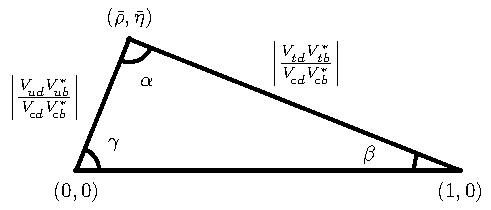
\includegraphics[scale=1.1]{diagram_ut}
  \end{center}
  \caption[Schematic diagram of the Unitarity Triangle]
  {
    Schematic diagram of the Unitarity triangle given in Eq.~\protect\ref{eq:th:ut} on the complex
    plane, where the base has been normalised to unit length.
    The angles $\alpha$, $\beta$, and $\gamma$ are defined in Eq~\protect\ref{eq:ut:angles}.
  }
  \label{fig:th:ut}
\end{figure}


Each \ckm matrix element is a fundamental parameter in the \sm, \replaced{it is}{and is} therefore important to
measure them all; particularly because the \ckm matrix holds all
%Precise determination of the \ckm matrix elements is important, for  they are each fundamental
%parameters of the SM.
%They also contain all the information about flavour violation and \CPV that is allowed within the
the information about flavour violation and \CPV \deleted{that is} allowed within the
framework of the quark sector of the \sm.
All the measurements relating to the \ckm matrix can be shown in the \ut.
%Current measurements of angles and side lengths from \Ref{Charles:2015gya} are shown in
%\Fig{fig:th:ckmfitter}.








%%&spell
\section{Physics beyond the Standard Model}
\label{sec:bsm}

For a long time the completion of the \sm was reliant on the discovery of the Hiigs boson.
Finally, in 2012, the \cms~\cite{Chatrchyan:2008aa} and \atlas~\cite{Aad:2008zzm} detectors
observed a Higgs boson with a mass of $m_H\simeq125\gev$~\cite{Chatrchyan:2012ufa,Aad:2012tfa}.
This final piece of the picture has made the \sm a remarkably robust theory with no predictions
deviating significantly from experimental observations.
Indeed, the theory of \QED~--- which describes interactions between
photons and charged particles in the \sm --- is one of the most accurate theories yet constructed.
The coupling constant in \QED is the fine structure constant, $\alpha$, which has been measured
experimentally to be~\cite{PDG2012}
\begin{align}
  \alpha^{-1}_\mathrm{exp} &= 137.035\,999\,074\,(44), \nonumber\\
  \intertext{and predicted theoretically to be~\cite{Aoyama:2012wj}}
  \alpha^{-1}_\mathrm{th} &= 137.035\,999\,073\,(35), \nonumber
\end{align}
%\begin{align}
  %\phantom{.} &&\alpha^{-1}_\mathrm{exp} &= 137.035\,999\,074\,(44), && \text{\cite{PDG2012}} \nonumber\\
  %\intertext{cats are the best}
  %\phantom{.} &&\alpha^{-1}_\mathrm{th} &= 137.035\,999\,073\,(35), && \text{\cite{Aoyama:2012wj}}
%\end{align}
with precisions better than one part per billion.


%Indeed, the fine structure constant, $\alpha$, which characterizes the coupling strength of
%electromagnetic interactions
%% is one of the most accurately predicted physical values.  The value of $\alpha^{-1}$
%is measured to be:
%\begin{equation}
  %\alpha^{-1} = 137.035\,999\,074\,(44),
%\end{equation}
%with a relative uncertainty of 0.32 parts per billion~\cite{PDG2012}.
%While the current best theoretical prediction, which accounts for up to tenth order Feynman
%diagrams, is:
%\begin{equation}
  %\alpha^{-1} = 137.035\,999\,073\,(35),
%\end{equation}
%to an accuracy of 0.25 parts per billion~\cite{Aoyama:2012wj}.
%Agreement between such precisely measured values, makes the theory of Quantum Electrodynamics,
%which describes interactions of photons and charged particles in the \sm, one of the most accurate
%theories yet constructed.

Despite its countless successes, there are a plethora of indications --- both
experimental and theoretical --- that additional physics exists, \bsm.



\subsection{Failures and inconsistencies of the Standard Model}
\label{sec:bsm:fail}
%%%%%%%%%%%%%%%%%%%%%%%%%%%%%%%%%%%%%%%%%%%%%%%%%%%%%%%%%%%%%%%%%%%%%%%%%%%%%%%%%%%%%%%%%%%%%%%%%%%
% Experimental
%%%%%%%%%%%%%%%%%%%%%%%%%%%%%%%%%%%%%%%%%%%%%%%%%%%%%%%%%%%%%%%%%%%%%%%%%%%%%%%%%%%%%%%%%%%%%%%%%%%
There are some phenomena that have been observed experimentally which cannot be explained by the
\sm.
Oscillations of neutrinos in flavour space mean that they must have mass; this is not accounted for
the \sm framework.
Neither are the observations of the \BAU and \dm.

% CPV
The \sm cannot reconcile the matter-antimatter asymmetry observed in the
Universe today.
The hypothesized process which caused this asymmetry is known as baryogenesis.
Whatever this process may be it must satisfy the three Sakharov
conditions~\cite{1991SvPhU..34..392S} which outline minimum requirements for baryogenesis.
The first, most obvious, criteria is that baryogenesis must violate baryon number.
The second Sakharov condition is that both \gls{C} and \CP are violated.
Lastly, baryogenesis must occur out of thermal equilibrium.
While the \sm does contain \CPV, it is approximately ten orders of
magnitude~\cite{Cline:2006ts,Huet:1994jb} too small to explain the \BAU.
%Other pressing problems in the \sm are that it cannot reconcile massive neutrinos, gravity, or the
%amount of mass that is not accounted for in the Universe.
In \Chap{ch:dsphi} a measurement of the \CP-asymmetry in the decay \btodsphi is made in an effort
to explain the \BAU.




% DARK MATTER
It is well known that the vast majority of mass in the Universe is unaccounted for.
Luminous matter totals only \approx$4.9\pc$ of the Universe~\cite{Adam:2015rua,PDG2014}, and the rest
is known only as \dm (\approx$26.8\pc$) and dark energy (\approx$68.3\pc$).
Dark Matter is an old and well motivated concept with the first evidence found in 1939 by H.~W.~Babcock
in the form of flat galactic rotation curves~\cite{1970ApJ...159..379R,1980ApJ...238..471R}.
Since then, corroborating evidence from, for example, gravitational lensing around the Bullet
cluster~\cite{Markevitch:2003at} has given further credence to its existence.

%The above observations clearly indicate that the \sm is not the complete picture of particle
%physics; but there are also some conflicts in more recent measurements that might hint at \np.

The theory of \SUSY naturally supplies a \dm candidate in the shape of the lightest supersymmetric particle,
which is stable because of the imposed conservation of $R$-parity.
\SUSY is a theory which introduces an additional super-particle for each \sm fermion and
gauge boson, whose spin differs by a half integer.
The Higgs sector in \SUSY comprises four Higgs doublets; two are spin-0 and two are spin-$\tfrac12$,
and then there are two each for $Y=\pm\tfrac12$.
After \SUSY is broken there are five Higgs physical scalar particles, two are \CP-even ($h^0$,
$H^0$) one is \CP-odd scalar ($A^0$) and two are charged charged ($H^\pm$).
It also immediately solves the hierarchy problem because for every \sm particle that contributes to
the Higgs mass, a \SUSY particle also contributes, but with the opposite sign.
Unfortunately, masses of the super-particles are unconstrained, and could be anywhere between a few
TeV and the Planck scale.

Observations of \dm can also be used to motivate \bsm models which include dark sectors.
A dark sector is a name for a particle, or group of particles, which is gauged under a
different gauge group to the \sm particles and therefore cannot interact with them directly.
There are a plethora of such models, but generally dark particles can only interact with the \sm
via weakly interacting messenger particles, which could be either vector or scalar.
In generality, these are known as \emph{Dark Bosons}.

Some excitement was caused by a hint of a dark sector messenger particle from the Hyper-\CP
experiment~\cite{Burnstein:2004uk}, which observes three $\decay{\Sigma^+}{p\mumu}$ events which
survive a stringent selection.
These three events also peak in the invariant mass of the dimuon pair.
The narrowness of this peak is indicative of a two body decay, consistent with  $\decay{\Sigma^+}{pP^0}$
and the subsequent decay of the \np particle via $\decay{P^0}{\mumu}$, where
$m_{P^0}=214.3\pm0.5\mev$~\cite{Park:2005eka}.
The $P^0$ could be the supersymmetric Goldstino, or a dark boson from many other theories.

\glspl{FCNC} are heavily suppressed in the \sm.
Firstly, they are forbidden at tree level; secondly, loop level diagrams are suppressed by factors
coming from the \ckm matrix.
These low background provide ideal environments to search for \bsm physics, since new massive
off-shell particles can contribute to the loops and cause significant deviations from \sm
expectations.

This thesis documents a search for a \np particle in the dimuon spectrum of \btokstrmumu in
\Chap{ch:db}.
Also detailed, in \Chap{db:hhh}, is an observation of a high statistics \fcnc decay in
\Chap{ch:hhh} which could be used for future \np searches.









%A hint at evidence for a \np particle comes from the Hyper-\CP experiment~\cite{Burnstein:2004uk}, which
%observes three $\decay{\Sigma^+}{p\mumu}$ events which survive a stringent selection.
%These three events also peak in the invariant mass of the dimuon pair.
%The narrowness of this peak is indicative of a two body decay, consistent with  $\decay{\Sigma^+}{pP^0}$
%and the subsequent decay of the \np particle via $\decay{P^0}{\mumu}$, where
%$m_{P^0}=214.3\pm0.5\mev$~\cite{Park:2005eka}.



%%%%%%%%%%%%%%%%%%%%%%%%%%%%%%%%%%%%%%%%%%%%%%%%%%%%%%%%%%%%%%%%%%%%%%%%%%%%%%%%%%%%%%%%%%%%%%%%%%%
% Theoretical
%%%%%%%%%%%%%%%%%%%%%%%%%%%%%%%%%%%%%%%%%%%%%%%%%%%%%%%%%%%%%%%%%%%%%%%%%%%%%%%%%%%%%%%%%%%%%%%%%%%
Theoretical shortcomings of the \sm include: its inability to incorporate gravity at the quantum
scale, the existence of dark energy.
However, theoretical reasons suggesting \bsm physics
are often rather subjective and revolve around the idea of \emph{naturalness}.
Naturalness is a concept whereby a theory is deemed to be natural, or more plausible, if it has few
free parameters, all of which have a magnitude $\mathcal{O}(1)$.
The \sm is not a natural theory.
For example: there are a total of 18 free parameters in the \sm, 13 of which reside in the flavour
sector;
The \ckm matrix is strongly hierarchic
%--- favouring flavour conserving weak interactions ---
and the quark masses vary by four orders of magnitude.

One of the fundamental parameters of the \sm  is \V{ub} and it is therefore important to accurately
measure it.
This parameter is particularly interesting because it is the source of the largest
tension in the \ut.
A determination of \V{ub} can be made using inclusive and exclusive measurements of semi-leptonic
$\decay{B}{X_u\ell\bar\nu_\ell}$ decays.
Inclusive measurements are made difficult by large
$\decay{B}{X_c\ell\bar\nu_\ell}$ backgrounds, while exclusive semi-leptonic modes suffer from
uncertainties introduced by form factors.
A value of $\left|\V{ub}\right|$ can also be obtained from the annihilation decay
$\decay{\Bp}{\taup\nu_\tau}$, but this suffers from low statistics.
Determinations of \V{ub} from these sources are:
\begin{align}
  &&\left|\V{ub}\right|_\mathrm{exc}
  &= \big(4.41\,^{+0.21}_{-0.23}\big)\e{-3}
  & \text{\cite{PDG2014}}& \nonumber\\
  &&\left|\V{ub}\right|_{\makebox[\widthof{$_\mathrm{exc}$}][l]{$_\mathrm{inc}$}}
  &= \big(3.28\pm{0.29}\big)\e{-3}
  & \text{\cite{PDG2014}}&\nonumber\\
  &&\left|\V{ub}\right|_{\makebox[\widthof{$_\mathrm{exc}$}][l]{$_{\tau\nu}$}}
  &= \big(4.22\pm{0.42}\big)\e{-3}  &
  \bam{Update} \text{\cite{PDG2012}}.&
  %%|\V{ub}| &= \big(4.22\pm{0.42}\big)\e{-3}  & \big(\decay{\Bp}{\taup\nu_\tau}\big)\text{\cite{{PhysRevD.88.031102}&\nonumber
  \label{eq:th:vub}
\end{align}
There are obvious tensions between the inclusive and exclusive modes, which could hint at some new
process.
A more accurate value of \V{ub} from the decay $\decay{\Bp}{\taup\nu_\tau}$ might shed light on the
situation.
Limits on \ut measurements are shown in \Fig{fig:th:ut}, and
global \V{ub} measurements from the semi-leptonic and $\decay{\Bp}{\taup\nu_\tau}$
modes are shown alongside one another.


Unnatural \np models with parameters which differ wildly in magnitude tend to
lead to parameters or processes that must cancel to absurdly
high precision in order to agree with experimental observations.
These precise cancellations are known as \emph{fine tuning}.
In the \sm, quantum loop corrections to the Higgs mass are of the order $10^{19}$
for $m_H\simeq125\gev$~\cite{Chatrchyan:2012ufa,Aad:2012tfa}.
This means that the cancellations required to result in a Higgs mass comparable to the masses of
the weak vector bosons must be exact to 17 orders of magnitude.
This instance of fine tuning is known as the \emph{hierarchy problem}.
A solution for the hierarchy problem would be to introduce NP particles, whose contributions to
loop level processes reduce the magnitude of fine tuning required to a level that might be deemed
expectable.

Fine tuning also appears in \QCD.
A gauge invariant term that can be added to \Lag{QCD} is
\begin{equation}
  \Lag{QCD}^\theta = \theta\frac{g^2}{32\pi^2}
  G_{\mu\nu}^\alpha\widetilde G^{\mu\nu}_\alpha,
  \label{eq:strongcp}
\end{equation}
where $\theta$ and $g$ are constants, and $\alpha$ indicates a sum over colours.
The operator $G_{\mu\nu}$ is the gluon field strength tensor, and
\begin{equation}
  \widetilde G^{\mu\nu}_\alpha = \frac12\varepsilon_{\mu\nu\rho\sigma}G^{\rho\sigma}_\alpha.
\end{equation}
Interactions in $\Lag{QCD}^\theta$ would conserve \gls{C} symmetry, but violate both \gls{P} and
\gls{T} conjugation~\cite{Peccei:2006as}.
Such symmetry violations are in contradiction with the observed properties of the strong
force.
Bounds placed on the value of the neutron dipole moment, $|d_n| <2.9\e{-26}\,\mathrm{ecm}$
(at 90\% CL)~\cite{Baker:2006ts} require $\theta$ to be very small,
$\theta<10^{-19}$~\cite{Crewther:PQref9}, when \emph{a priori} it could be in the range
$0<\theta<2\pi$.
This occurrence of fine tuning is referred to as the \emph{strong \CP problem}.


Despite the evidence for \bsm physics and the list of problems that must be solved, its precise
manifestation is unknown.
There are numerous theories concerning NP scenarios which seek to solve various problems.

New physics models accommodate \dm in different ways.
Some models have a \emph{dark} or \emph{hidden} sector which, apart from gravity, only
communicates with the visible sector feebly via messenger particles.
These messenger particles could potentially be observed after they decay into \sm particles after
mixing with a $H$, $Z$, $\gamma$ or $\nu$.
A solution to the strong \CP problem is to introduce an additional chiral symmetry, such that
$\theta$, in \Eq{eq:strongcp}, becomes a field: the quanta of which are called \emph{axions}.
These axions could be the messenger particle between the dark and visible
sectors~\cite{Peccei:2006as}.

%%%%%%%%%%%%%%%%%%%%%%%%%%%%%%%%%%%%%%%%%%%%%%%%%%%%%%%%%%%%%%%%%%%%%%%%%%%%%%%%%%%%%%%%%%%%%%%%%%
%%%%%%%%%%%%%%%%%%%%%%%%%%%%%%%%%%%%%%%%%%%%%%%%%%%%%%%%%%%%%%%%%%%%%%%%%%%%%%%%%%%%%%%%%%%%%%%%%%
%%%%%%%%%%%%%%%%%%%%%%%%%%%%%%%%%%%%%%%%%%%%%%%%%%%%%%%%%%%%%%%%%%%%%%%%%%%%%%%%%%%%%%%%%%%%%%%%%%




%%%%%%%%%%%%%%%%%%%%%%%%%%%%%%%%%%%%%%%%%%%%%%%%%%%%%%%%%%%%%%%%%%%%%%%%%%%%%%%%%%%%%%%%%%%%%%%%%%
%%%%%%%%%%%%%%%%%%%%%%%%%%%%%%%%%%%%%%%%%%%%%%%%%%%%%%%%%%%%%%%%%%%%%%%%%%%%%%%%%%%%%%%%%%%%%%%%%%
%%%%%%%%%%%%%%%%%%%%%%%%%%%%%%%%%%%%%%%%%%%%%%%%%%%%%%%%%%%%%%%%%%%%%%%%%%%%%%%%%%%%%%%%%%%%%%%%%%






Some searches look directly for evidence of NP, this is the case for the analysis detailed in
\Chap{ch:db}, where a new particle, \db, is searched for in the dimuon invariant mass spectrum of
\decay{\Bd}{\Kstarent\mumu} consistent with \decay{\db}{\mumu}.
This is sensitive to a range of models which predict a light particle with a mass in the range
$2m_\mu\lesssim m_\db\lesssim4000\mev$, such as the axion model.
It is also sensitive to the $P^0$ that was hinted at by the Hyper-\CP experiment.

Instead of counting on NP to behave in an expected way, it is possible to search in a model
independent manner by exploring general physics couplings.
To do this it is useful to introduce the \OPE~\cite{PhysRev.179.1499}.



%%\subsection{Uncertainties in theoretical predictions}
\section{Dealing with QCD}

For the branching fractions discussed in this thesis, theoretical uncertainties from \QCD make
predictions difficult\footnote{
  The following section is based on Refs.~\cite{Pich:1998xt}.
}.
Quantum Chromodynamics describes the interactions of colour charged particles (quarks and
gluons).
%interactions between quarks via the strong force which is mediated by gluons.
The behaviour of \QCD exhibits two peculiarities: confinement, and asymptotic freedom.
Confinement describes the strong force over long distances ($\approx1\fm$)
where, unlike QED, the interaction strength does not lessen with distance.
This means that as a quark is separated from others, there is enough energy in the gluon field to
create a new quark-antiquark pair.
The resulting bound states always have net zero colour charge.
Therefore, free quarks are never observed over macroscopic distances
and are observed as mesons (quark-antiquark bound states), baryons (bound states of
three quarks), or tetra-quarks~\cite{LHCb-PAPER-2014-014}.
%but are seen to behave as free
%particles in deep inelastic scattering.
Asymptotic freedom means that forces between quarks become asymptotically weaker as the energy of
the system increases --- and the distance decreases.

Predictions of $b$-hadron processes involving \QCD can also be made using effective field theory.
Despite the large mass of the \bquark quark with respect to $\Lambda_\mathrm{QCD}\simeq200\mev$,
the system can be treated perturbatively since $\alpha_\mathrm{QCD}(m_\bquark)$ is sufficiently
small.
This is known as a Heavy Quark Effective Theory (HQET).
In contrast to an EFT where the weak fields have been integrated out, in a HQET
it is not possible to remove heavy quark contributions entirely because the \bquark quark
cannot decay without violating flavour number.
This essentially treats a $b$-hadron like a hydrogen atom, where the \bquark quark takes
the place of the nucleus, allowing for a highly simplified theoretical treatment, with corrections
of order $m_\bquark^{-1}$.

Despite the use of HQET, the fact is that hadrons are inherently non-perturbative objects, and so
it is useful to make further assumptions.
An important supposition is that of \emph{factorization} which assumes that the short-distance,
process dependent, \QCD effects are separable from hadronization, the long distance effects.
Hadronization is very difficult to calculate with \QCD, for this reason form-factors are used to
empirically encapsulate the process.
Form-factors must be measured experimentally and are the dominant source of uncertainty in the
calculation of $B$ mesons decaying into hadronic (or semi-hadronic) final states.





%The mass of the \bquark quark is sufficiently high that QCD calculations in $B$ decays can be made
%using peturbation theory.
%Furthermore, initial conditions can modelled using Heavy Quark Effective Theory (HQET), which
%essentially models a bound state of a heavy and light quark like a hydrogen atom, with the \bquark
%taking the role of the nucleus.
%However, this latter approximation breaks down at low energies where the hadron has an energy
%comparable to the mass of the \bquark quark.

%Another important assumption for QCD predictions is that of factorizability.
%A decay is factorizable if one can separate the initial, partonic, state from the hadronization of
%the final state quarks.
%Hadronization is very difficult to model, and therefore empirical models, encoded into
%form-factors, are used.
%It is these form-factors which are the dominant source of theoretical uncertainty.


%These oddities mean that QCD must be dealt with in different ways depending on the energy regime of
%interest.
%For high momentum interations the coupling strength, $\alpha_\mathrm{QCD}$ is small and the system
%can be dealt with using peturbation theory.
%But, for low momentum interactions $\alpha_\mathrm{QCD}$ increases because of the
%\emph{running} of the coupling.
%In the latter regime the system cannot be modelled with peturbation theory because it is not
%infrared safe and rather Lattice QCD must be used.
%Another inadequacy of peturbation theory is that it considers asymptotic states of quarks and
%gluons as free states, where in actuallity the physical states which are observed are hadrons.
%
%Difficulties with calculating QCD interactions leads to the necessity of form factors, which are
%empirical functions with parameters measured experimentally.
%These are
%
%
%\begin{itemize}
  %\item Heavy quark effective field theory simpolify calculations
    %interactions of the heacy wuark are soft cmopared tot the large mass of the $B$, and partonic
    %process is expanded in terms of $\Lambda_{QCD}/m_B$
  %\item QCD factorization setarates partonic process from the hadronisation of the $sq$ pair
  %\item Hadronisation is encoded into hadronic form-factors which is the dominant source of
    %uncertainty for theoretical predictions
%\end{itemize}









\begin{minipage}{\textwidth}
  {\it ``Before beginning a Hunt, it is wise to ask someone what you are looking for before you
  begin looking for it.''}

  {\hfill Winnie the Pooh, A.A.~Milne}
\end{minipage}

\vspace{2em}

This thesis contains the work undertaken in three analyses; each of which concerns a different area
of interest in \gls{HEP}.
The following chapter aims to motivate each analysis in turn after introducing the Standard Model
of particle physics.

Firstly, the formulation of the \sm will be outlined, with particular detail paid to the flavour
sector.
Various successes of the \sm will then be discussed before going on to identify its shortcomings
using arguments from both experiment and theory.
These shortcomings will then be used to motivate the three analyses:
a search for the decay \btodsphi (\Chap{ch:dsphi});
a search for the two related decays \btokpipimumu and \btophikmumu (\Chap{ch:hhh});
a search for dark sector particles in $\decay{\Bd}{K^*(892)^0}$ (\Chap{ch:db}).
Theory specific to each of these analyses will be detailed in the relevant chapter.

%The convension of natural units, $c=\hbar=1$, is assumed throughout.
%Indices for four vectors are labelled by $\mu$ and $\nu$, and indices for the $SU_C(3)$ and
%$SU_L(2)$ generators are

%The following chapter will elucidate as to how the flavour sector is the only source of \CPV in the
%SM.
%It will then go on to motivate study of flavour physics at \lhcb by exploring some problems with
%the SM as a theory.

\section{The Standard Model}
The current formulation of the SM of particle physics was concocted in the 1970s, when the Higgs
mechanism was incorporated into Glashow's electroweak theory by Salam and Weinberg.
The theory prescribes a treatment
as to how fundamental particles interact via three of the four
fundamental forces, namely: the strong, weak and electromagnetic forces.

%Mathematically, the SM is a locally gauge invariant quantum field theory, where excitations of
%various fields manifest themselves as particles.
%There is a global Poincare symmetry as required by special relativity; and a local
%$SU(3)\times SU(2)\times U(1)$ symmetry which encapsulates the SM Lagrangian:
%\begin{equation}
  %\Lag{SM} = \Lag{EW} + \Lag{Strong} + \Lag{Higgs}.
%\end{equation}
%Where the components describe the electroweak, strong and Higgs interactions.
%Each generator of this local gauge group is associated with a gauge boson which mediates
%interactions between other bosons and fermions.

Mathematically, the SM is a locally gauge invariant quantum field theory.
It inhabits a space-time with a global Poincar\'e symmetry that obeys a local
$SU(3)\times SU(2)\times U(1)$ symmetry.
Each generator in this group corresponds to a gauge-boson; so the strong force ($SU(3)$ group) has
eight gluons that mediate the interaction, and the electroweak force ($SU(2)\times U(1)$ group) has
$3+1$ gauge bosons, which are the weak gauge bosons ($Z$, $W^\pm$) and the photon ($\gamma$).
These are all vector fields.
Fermions are described by spinor fields, $\psi$, which obey the Dirac equation:
\begin{equation}
  (i\hbar\gamma^\mu\partial_\mu - mc)\psi = 0.
  \label{th:eq:dirac}
\end{equation}
The fermions of the SM constitute six leptons (electron, electron neutrino, muon, muon neutrino,
tau and tau neutrino) and six quarks (up, down, charm, strange, top and bottom), which are
organized into pairs forming three generations.
For each fermion there is a corresponding antiparticle with the same mass and opposite charge ---
charge being the conserved quantity resulting from the global gauge symmetry (by Noether's
theorem).
There is also a single scalar field in the SM, that of the Higgs boson.
%The only additional particle is the scalar Higgs boson.

The SM Lagrangian can be expressed as a sum of components:
\begin{equation}
  \Lag{SM} = \Lag{QCD} + \Lag{V} + \Lag{\ell} + \Lag{\it q} + \Lag{Higgs} + \Lag{Yuk}.
  \label{eq:th:lag}
\end{equation}
The first term describes interactions of the strong force between colour carrying particles in the
theory of Quantum Chromodynamics (QCD).
Descriptions of weak vector boson self-interactions, and the electroweak behavior of
leptons are encapsulated in the next two terms.
Finally, the remaining terms describe the electroweak behavior of quarks, the Higgs interaction and Yukawa
couplings, respectively.
These latter terms are of fundamental importance as to how flavour changing currents and CPV
occur in the SM. %, and will be be discussed in detail.
%the SM.
%Each of these shall be discussed in turn.

%\subsection{Uncertainties in theoretical predictions}
\section{Dealing with QCD}

For the branching fractions discussed in this thesis, theoretical uncertainties from \QCD make
predictions difficult\footnote{
  The following section is based on Refs.~\cite{Pich:1998xt}.
}.
Quantum Chromodynamics describes the interactions of colour charged particles (quarks and
gluons).
%interactions between quarks via the strong force which is mediated by gluons.
The behaviour of \QCD exhibits two peculiarities: confinement, and asymptotic freedom.
Confinement describes the strong force over long distances ($\approx1\fm$)
where, unlike QED, the interaction strength does not lessen with distance.
This means that as a quark is separated from others, there is enough energy in the gluon field to
create a new quark-antiquark pair.
The resulting bound states always have net zero colour charge.
Therefore, free quarks are never observed over macroscopic distances
and are observed as mesons (quark-antiquark bound states), baryons (bound states of
three quarks), or tetra-quarks~\cite{LHCb-PAPER-2014-014}.
%but are seen to behave as free
%particles in deep inelastic scattering.
Asymptotic freedom means that forces between quarks become asymptotically weaker as the energy of
the system increases --- and the distance decreases.

Predictions of $b$-hadron processes involving \QCD can also be made using effective field theory.
Despite the large mass of the \bquark quark with respect to $\Lambda_\mathrm{QCD}\simeq200\mev$,
the system can be treated perturbatively since $\alpha_\mathrm{QCD}(m_\bquark)$ is sufficiently
small.
This is known as a Heavy Quark Effective Theory (HQET).
In contrast to an EFT where the weak fields have been integrated out, in a HQET
it is not possible to remove heavy quark contributions entirely because the \bquark quark
cannot decay without violating flavour number.
This essentially treats a $b$-hadron like a hydrogen atom, where the \bquark quark takes
the place of the nucleus, allowing for a highly simplified theoretical treatment, with corrections
of order $m_\bquark^{-1}$.

Despite the use of HQET, the fact is that hadrons are inherently non-perturbative objects, and so
it is useful to make further assumptions.
An important supposition is that of \emph{factorization} which assumes that the short-distance,
process dependent, \QCD effects are separable from hadronization, the long distance effects.
Hadronization is very difficult to calculate with \QCD, for this reason form-factors are used to
empirically encapsulate the process.
Form-factors must be measured experimentally and are the dominant source of uncertainty in the
calculation of $B$ mesons decaying into hadronic (or semi-hadronic) final states.





%The mass of the \bquark quark is sufficiently high that QCD calculations in $B$ decays can be made
%using peturbation theory.
%Furthermore, initial conditions can modelled using Heavy Quark Effective Theory (HQET), which
%essentially models a bound state of a heavy and light quark like a hydrogen atom, with the \bquark
%taking the role of the nucleus.
%However, this latter approximation breaks down at low energies where the hadron has an energy
%comparable to the mass of the \bquark quark.

%Another important assumption for QCD predictions is that of factorizability.
%A decay is factorizable if one can separate the initial, partonic, state from the hadronization of
%the final state quarks.
%Hadronization is very difficult to model, and therefore empirical models, encoded into
%form-factors, are used.
%It is these form-factors which are the dominant source of theoretical uncertainty.


%These oddities mean that QCD must be dealt with in different ways depending on the energy regime of
%interest.
%For high momentum interations the coupling strength, $\alpha_\mathrm{QCD}$ is small and the system
%can be dealt with using peturbation theory.
%But, for low momentum interactions $\alpha_\mathrm{QCD}$ increases because of the
%\emph{running} of the coupling.
%In the latter regime the system cannot be modelled with peturbation theory because it is not
%infrared safe and rather Lattice QCD must be used.
%Another inadequacy of peturbation theory is that it considers asymptotic states of quarks and
%gluons as free states, where in actuallity the physical states which are observed are hadrons.
%
%Difficulties with calculating QCD interactions leads to the necessity of form factors, which are
%empirical functions with parameters measured experimentally.
%These are
%
%
%\begin{itemize}
  %\item Heavy quark effective field theory simpolify calculations
    %interactions of the heacy wuark are soft cmopared tot the large mass of the $B$, and partonic
    %process is expanded in terms of $\Lambda_{QCD}/m_B$
  %\item QCD factorization setarates partonic process from the hadronisation of the $sq$ pair
  %\item Hadronisation is encoded into hadronic form-factors which is the dominant source of
    %uncertainty for theoretical predictions
%\end{itemize}








%The following chapter will elucidate as to how the flavour sector is the only source of CPV in the
%SM.
The structure of CP and flavour violation emerges as a direct consequence of the Higgs mechanism
breaking the local electroweak symmetry.
The Lagrangian of the scalar Higgs field is:
\begin{align}
  \Lag{Higgs}
  &= \left(D_\mu\Phi\right)^\dagger\left(D^\mu\Phi\right) - V(\Phi) \\
  &= \left(D_\mu\Phi\right)^\dagger\left(D^\mu\Phi\right) - \mu^2\left(\Phi^\dagger\Phi\right) +
  \lambda\left(\Phi^\dagger\Phi\right),
  \label{eq:th:laghiggs1}
\end{align}
where $\mu$ and $\lambda$ are constants, $D_\mu$ is the covariant derivative, and $\Phi$ is the
Higgs doublet, defined by:
\begin{equation}
  \Phi = \frac{1}{\sqrt{2}}
  \begin{pmatrix}
    \phi_1 + i\phi_2 \\
    \phi_3 + i\phi_4 \\
  \end{pmatrix}.
  \label{eq:th:phi}
\end{equation}
Taking $\mu^2<0$ and $\lambda>0$ moves the minimum of the potential $V(\Phi)$ away from zero to a distance $v$:
\begin{equation}
  v = \sqrt{\frac{\mu^2}{\lambda}}.
\end{equation}
At this point the Higgs field gets a vacuum expectation value (VEV)
%$\braket{\phi} = \tfrac{1}{\sqrt{2}}v$.
of $\langle\phi\rangle = \tfrac{1}{\sqrt{2}}v$.
The direction of the VEV from the origin is arbitrary, but the choice of:
\begin{align}
  \bra{0}\phi_1\ket{0} =
  \bra{0}\phi_2\ket{0} =
  \bra{0}\phi_4\ket{0} = 0  &&
  \bra{0}\phi_3\ket{0} = v,
\end{align}
is convenient, and changes Eq.~\ref{eq:th:phi} to:
\begin{equation}
  \Phi = \frac{1}{\sqrt{2}}
  \begin{pmatrix}
    \eta_1 + i\eta_2 \\
    v + i\eta_4 \\
  \end{pmatrix}.
  \label{eq:th:eta}
\end{equation}
Here, $\eta_1$, $\eta_2$ and $\eta_4$, are Goldstone bosons which, by choosing an appropriate
gauge, become the longitudinal components of the weak bosons.
This choice of gauge simplifies $\Phi$ to:
\begin{equation}
  \Phi =
  \begin{pmatrix} 0 \\ v+H
  \end{pmatrix},
  \label{eq:th:phi2}
\end{equation}
where $H$ is the physical Higgs boson.
%Using this in Eq.~\ref{eq:th:laghiggs1} gives:
Inserting Eq.~\ref{eq:th:phi2} into Eq.~\ref{eq:th:laghiggs1} gives:
%\begin{multline}
  %\Lag{Higgs} =
  %\frac12\left(\partial_\mu H\right)\left(\partial^\mu H\right)
  %+\frac14g^2\left(v^2 + 2vH + H^2\right)W_\mu^+W^{-\mu}  \\
  %+\frac18\left(g^2 + g^{\prime2}\right)\left(v^2 + 2vH + H^2\right)Z_\mu Z^\mu
  %+ \mu^2H^2 + \frac14\lambda\left(H^4+4vH^3\right) + \cdots,
  %\label{eq:th:laghiggs2}
%\end{multline}
\begin{equation}
  \Lag{Higgs} =
  \frac12\left(\partial_\mu H\right)\left(\partial^\mu H\right)
  +\mu^2H^2
  +\left(m_W^2W_\mu^+W^{-\mu} + \frac{m_Z^2}{2}Z_\mu Z^\mu\right)
  \cdot
  \left(1 + \frac{H}{v}\right)^2
  \label{eq:th:laghiggs2}
\end{equation}
where $g$ and $g^\prime$ are coupling constants and other terms are three- and four-point
interactions of the Higgs with itself and weak gauge bosons.
Thus, the $U(1)$ local gauge symmetry is broken, weak gauge boson acquire a mass while photons remain
massless; as is consistent with observations.


%It is not possible to directly insert mass terms for fermions, because the required terms
%($m(\bar\psi_L\psi_R+\bar\psi_R\psi_L$) are not allowed \bam{ELABORATE}.
All fermions (except neutrinos) also get a mass after the spontaneous symmetry breaking (SSB) of
the $U(1)$ symmetry.
The Dirac mass term for a chiral field should be of the form:
\begin{equation}
  \Lag{mass} = -m_\psi\left(\bar\psi_R\psi_L + \bar\psi_L\psi_R\right),
\end{equation}
but the left- and right-handed fields have different $U(1)$ charges %Y hypercharge
and so transform differently under local gauge transformations and so cannot be added to \Lag{SM}.
However, masses can be generated through the Yukawa couplings (\Lag{Yuk} in \Eq{eq:th:lag}), which
describe integrations between all fermionic fields and the Higgs doublet, and can be written:
\begin{equation}
  \Lag{Yuk} = \sum_{\substack{\ell=\\e,\mu,\tau}}\left(\Lag{Yuk}^\ell\right) + \Lag{Yuk}^q,
  \label{eq:th:yukking}
\end{equation}
where $\ell$ and $q$ denote the lepton and quark sectors respectively.
First considering the lepton term, after SSB:
\begin{align}
  \Lag{Yuk}^\ell
  &= - g_\ell\left(\bar\chi_L\Phi \ell_R + \bar \ell_R\Phi^\dagger\chi_L\right) \\
  &= - \frac{g_\ell v}{\sqrt{2}}\left(\bar\ell_L\ell_R + \bar\ell_R\ell_L\right)\cdot
  \left(1 + \frac{H}{v}\right)
     %- \frac{g_\ell}{\sqrt{2}}H\left(\bar\ell_L\ell_R + \bar\ell_R\ell_L\right),
\end{align}
where $g_\ell$ is a coupling constant, and
\begin{align}
  \chi_L = \begin{pmatrix}\nu_L \\ \ell_L \end{pmatrix}.
\end{align}
Thus the leptons get a mass of $m_\ell = \tfrac{1}{\sqrt{2}}g_\ell v$, and interact with the Higgs
field.

The story for $\Lag{Yuk}^q$ is a bit more involved.
Before SSB:
\begin{align}
  \Lag{Yuk}^q &= - y_{ij}^u\bar Q_L^i\Phi u_R^j
  - y_{ij}^d\bar Q_L^i\tilde\Phi d_R^j + \mathrm{h.c.},
  \label{eq:th:lagyukq}
\end{align}
where there is an implicit sum over all generations $i$ and $j$, $y^{u,d}$ is a $3\times3$ matrix
characterizing the Yukawa couplings between quark generations,
\begin{align}
  \tilde\Phi_i &= \varepsilon_{ij}\Phi_j,
    \qquad \mathrm{and} \quad Q_L = \begin{pmatrix}u_L \\ d_L \end{pmatrix}.
\end{align}
After SSB, and the Higgs acquires a VEV, \Eq{eq:th:lagyukq} becomes:
\begin{equation}
  \Lag{Yuk}^q =
  - \frac{v}{\sqrt{2}}
  \left(
  y_{ij}^u\bar u_L^iu_{R,j}
  + y_{ij}^d\bar d_L^id_{R,j},
  + \mathrm{h.c.}
  \right)
  \cdot
  \left(1 + \frac{H}{v}\right),
  \label{eq:th:lagyuk2}
\end{equation}
where the mass of the quarks is $m_q = \frac{v}{\sqrt{2}}y_{ij}^q$.
However, it is more convenient to change a basis in which the matrix $m^q$ is diagonal such that
$m_{ij}^\mathrm{diag} = V_{Lik}m_{kl}(V_R^\dagger)_{lj}$.
This is exactly equivalent to transforming the chiral quark fields for up- and down-type quarks
accordingly:
\begin{align}
  q_L^\alpha = \left(V_L^q\right)_{\alpha i}q_L &&
  q_R^\alpha = \left(V_R^q\right)_{\alpha i}q_R,
\end{align}
where the index of the original basis is identified with $i$ and the mass basis uses $\alpha$.

The rotations of the basis of the chiral quark fields leave much of \Lag{SM} unchanged since
$V_{qL}^\dagger V_{qL} = V_{qR}^\dagger V_{qR} = \mathbb{1}$.
However, this is not the case in the charged current (CC) part of \Lag{\it q}; which transforms as:
\begin{align}
  \Lag{\it q}^\mathrm{CC}
  &= \frac{g}{2}i\gamma^\mu
  \left[\bar u_Ld_LW^+_\mu + \bar d_Lu_LW^-_\mu
  \right]  \\
  &= \frac{g}{2}i\gamma^\mu
  \left[
    \bar u_L\left(V_{uL}V_{dL}^\dagger\right)d_LW^+_\mu +
    \bar d_L\left(V_{dL}V_{uL}^\dagger\right)u_LW^-_\mu
  \right]  \\
  &= \frac{g}{2}i\gamma^\mu
  \left[
    V\bar u_Ld_LW^+_\mu +
    V^\dagger\bar d_Lu_LW^-_\mu
  \right].
\end{align}
The matrix $V$ is defined is known as the Cabibbo-Kobayashi-Maskawa (CKM) matrix
and parameterizes the couplings between up- and down-type quarks in charged weak currents.





\subsection{The CKM matrix and Unitarity Triangle}
\label{sec:ckm}

The \ckm matrix is defined as:
\begin{equation}
  \VCKM = \left(V_{uL}^{\phantom{\dagger}} V_{dL}^\dagger\right) =
  \begin{pmatrix}
    \V{ud} & \V{us} & \V{ub} \\
    \V{cd} & \V{cs} & \V{cb} \\
    \V{td} & \V{ts} & \V{tb} \\
  \end{pmatrix},
\end{equation}
where each $|V_{ij}|$ parameterises the probability of an up-type quark, of generation $i$,
transitioning to down-type quark, $j$, in a weak interaction.
In the \sm, it is assumed that the total charged current couplings of up- to down-type quarks is the
same as down- to up-type.
This means that the \ckm matrix is unitary, $\VCKMconj\VCKM = \mathds{1}$, and therefore it contains
only four physical parameters: three angles ($\theta_{12}$, $\theta_{13}$ and $\theta_{23}$) and one
complex phase ($\delta$).
In fact, the observation of \CPV in kaon mixing~\cite{Christenson:1964fg}
led to the prediction of a third generation before
its discovery, precisely because a $3\times3$ matrix is the smallest necessary for a phase to enter
a unitary matrix.

%preferentially
%hierarchichal
%arbiatry

%The CKM matrix is the source of all flavour violation in the SM.
%In the SM, it is assumed that the total charged current couplings of up- to down-type quarks is the
%same as down- to up-type.
%This means that the CKM matrix is unitary, $V^\dagger V = \mathbb{1}$, and therefore it contains
%four physical parameters: three angles ($\theta_{12}$, $\theta_{13}$ and $\theta_{23}$) and one
%complex phase ($\delta$).

%\begin{equation}
  %\VCKM =
  %\begin{pmatrix}
    %\cxx{12}\cxx{13} & \sxx{12}\cxx{13} & \sxx{13}e^{-i\delta} \\
    %-\sxx{12}\cxx{23}-\cxx{12}\sxx{23}\sxx{13}e^{i\delta} &
    %\cxx{12}\cxx{23}-\sxx{12}\sxx{23}\sxx{13}e^{i\delta} & \sxx{23}\cxx{13} \\
    %\sxx{12}\sxx{23}-\cxx{12}\cxx{23}\sxx{13}e^{i\delta} &
    %-\cxx{12}\sxx{23}-\sxx{12}\cxx{23}\sxx{13}e^{i\delta} & \cxx{23}\cxx{13} \\
  %\end{pmatrix}
%\end{equation}

There are many ways of representing the \ckm matrix.
One way is as a product of three rotation
matrices, one of which contains the complex phase, this is known as the \emph{standard}
parameterisation:
\begin{equation}
  \VCKM =
  \begin{pmatrix}
    \cxx{12}\cxx{13} & \sxx{12}\cxx{13} & \sxx{13}e^{-i\delta} \\
    -\sxx{12}\cxx{23}-\cxx{12}\sxx{23}\sxx{13}e^{i\delta} &
    \cxx{12}\cxx{23}-\sxx{12}\sxx{23}\sxx{13}e^{i\delta} & \sxx{23}\cxx{13} \\
    \sxx{12}\sxx{23}-\cxx{12}\cxx{23}\sxx{13}e^{i\delta} &
    -\cxx{12}\sxx{23}-\sxx{12}\cxx{23}\sxx{13}e^{i\delta} & \cxx{23}\cxx{13} \\
  \end{pmatrix},
\end{equation}
where $\sxx{ij}$ and $\cxx{ij}$ denote $\sin\theta_{ij}$ and $\cos\theta_{ij}$, respectively.
A convenient simplification is the \emph{Wolfenstein} parameterisation, which is obtained by
defining
\begin{align}
  \sin\theta_{12}&=\lambda, \nonumber\\
  \sin\theta_{23}&=A\lambda^2, \nonumber\\
  \intertext{and}
  e^{-i\delta}\sin\theta_{13} &= A\lambda^3(\rho-i\eta),
\end{align}
which results in
\begin{align}
  \VCKM\simeq
  \begin{pmatrix}
      %1-\tfrac12\lambda & \lambda & A\lambda^3(\rho-i\eta+\tfrac{i}2\eta\lambda^2) \\
      %-\lambda & 1-\lambda^2-i\eta A^2\lambda^4 & A\lambda^2(1+i\eta\lambda^2) \\
      %A\lambda^3(1-\rho-i\eta) & -A\lambda^2 & 1 \\
    1-\tfrac12\lambda & \lambda & A\lambda^3\big(\rho-i\eta\big) \\
    -\lambda & 1-\lambda^2 & A\lambda^2 \\
    A\lambda^3\big(1-\rho-i\eta\big) & -A\lambda^2 & 1 \\
  \end{pmatrix}.
  \label{eq:th:wolfenstein}
\end{align}
The values of the Wolfenstein parameters $A$ and $\lambda$ are:
\begin{spacing}{.8}
%{%
  %\setlength{\belowdisplayskip}{4pt}%
  %\setlength{\abovedisplayskip}{4pt}%
  \begin{align*}
  %\lambda &= 0.22537\pm0.00061, \nonumber\\\intertext{cat} A&=0.814\,^{+0.023}_{-0.024}.
    \lambda &= 0.22537\pm0.00061,
    \intertext{and}
    A&=0.814\,^{+0.023}_{-0.024}.
  \end{align*}
\end{spacing}
%}
Since $A\neq0$ and $\lambda\neq0$, it is clear that \VCKM is not diagonal, and therefore
flavour-changing currents are allowed in the \sm.
However,
it is most probable that a weak interaction is intra-generational, meaning that
the \ckm matrix exhibits a strongly hierarchic structure.
%However, the diagonal elements are close to unity and the CKM matrix exhibits a strong
%hierarchical structure, such that it is most probable that weak currents do not violate flavour.
%for which there is no explaination in the SM.


It has been asserted that the \ckm matrix is unitary, and therefore a
unitarity condition can be expressed as
$\Vconj{\alpha\beta}\V{\beta\gamma}=\delta_{\alpha\gamma}$.
%$V_{\alpha\beta}^{\phantom{\dagger}}V_{\beta\gamma}^* = \delta_{\alpha\gamma}$
%\begin{equation}
  %V_{\alpha\beta}^{\phantom{\dagger}}V_{\beta\gamma}^* = \delta_{\alpha\gamma},
  %\boldsymbol{V}_{ij}\boldsymbol{V}_{jk}^\dagger = \delta_{ik}.
  %\sum_{i=1}^3\left|V_{ij}\right|^2 = 1
  %\sum_{i=1}^3\left(V_{ij}^*V_{jk}\right) = \mathbb{1},
  %\label{eq:th:unitarity}
%\end{equation}
When $\delta_{\alpha\gamma}=0$, this condition gives six equations of the form:
\begin{align}
  %\sum_{i=1}^3V_{ij}^*V_{ki} &= 0 && \sum_{i=1}^3V_{ji}^*V_{ik} =0, & j&\neq k;
  \phantom{\beta\neq\gamma}
  &&\sum_{\beta=1}^3V_{\alpha\beta}^*V_{\beta\gamma}^{\phantom{*}} = 0,
  &&\sum_{\beta=1}^3V_{\alpha\beta}^{\phantom{*}}V_{\beta\gamma}^*=0,
  &&\alpha\neq\gamma;
  \label{eq:th:offdiag}
\end{align}
each mapping a closed \replaced{triangle}{triangles} on the complex plane.
Two of these triangles have all sides of similar length
%One of these triangles, which has sides of similar length
$\big(\mathcal{O}(\lambda^3)\big)$,
one of these is
is known as \emph{the} \ut and is defined by
%Taking the equations of the triangles in Eq.~\ref{eq:th:unitarity} where all sides have length of
%$\mathcal{O}(\lambda^3)$ leaves two triangles, one of which is:
\begin{equation}
  %\V{ud}\Vconj{ub} + \V{cd}\Vconj{cb} + \V{td}\Vconj{tb} = 0.
  1 + \frac{\V{ud}\Vconj{ub}}{\V{cd}\Vconj{cb}} + \frac{\V{td}\Vconj{tb}}{\V{cd}\Vconj{cb}} = 0,
  \label{eq:th:ut}
\end{equation}
where the length of the base has been normalised to unity.
The apex of the \ut is at
\begin{align}
  %\bar\rho+i\bar\eta = (1-\tfrac12\lambda^2)(\rho+i\eta)
  \xbar\rho+i\xbar\eta &= \big(1-\tfrac12\lambda^2\big)\big(\rho+i\eta\big)
  \nonumber\\
  &=\frac{\V{ud}\Vconj{ub}}{\V{cd}\Vconj{cb}},
\end{align}
%If divided through by $\V{cd}\Vconj{cb}$, then Eq.~\ref{eq:th:ut} can be mapped onto the complex
%plane, where the apex is at $\bar\rho+i\bar\eta = (1-\tfrac12\lambda^2)(\rho+i\eta)$.
%and the angles are
and forms the angles
\begin{align}
  \alpha &= \arg\left(-\frac{\V{td}\Vconj{tb}}{\V{ud}\Vconj{ub}}\right), &
  \beta  &= \arg\left(-\frac{\V{cd}\Vconj{cb}}{\V{td}\Vconj{tb}}\right), &
  \gamma &= \arg\left(-\frac{\V{ud}\Vconj{ub}}{\V{cd}\Vconj{cb}}\right).
  %\alpha &=    \arg\left(-\frac{\V{td}\Vconj{tb}}{\V{ud}\Vconj{ub}}\right), \nonumber\\
  %\beta  &=\pi-\arg\left( \frac{\V{td}\Vconj{tb}}{\V{cd}\Vconj{cb}}\right), \nonumber\\
  %%& &\mathrm{and}
  %\gamma &=    \arg\left( \frac{\V{ud}\Vconj{ub}}{\V{cd}\Vconj{cb}}\right).
  \label{eq:ut:angles}
\end{align}
which define phase differences between edges.
Figure~\ref{fig:th:ut} depicts a schematic diagram of the \ut.
%are phases between CKM matrix elements.
%This triangle is depicted in \Fig{fig:th:ut}.
%, is simply a graphical representation of the CKM matrix.
%Measurements of CKM matrix elements constrain the angles, side lengths and apex of the UT, these
%constraints are also shown in Fig.~\ref{fig:th:ut}.

\begin{figure}
  \begin{center}
      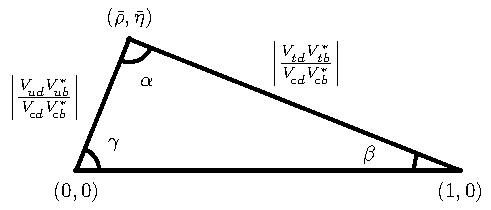
\includegraphics[scale=1.1]{diagram_ut}
  \end{center}
  \caption[Schematic diagram of the Unitarity Triangle]
  {
    Schematic diagram of the Unitarity triangle given in Eq.~\protect\ref{eq:th:ut} on the complex
    plane, where the base has been normalised to unit length.
    The angles $\alpha$, $\beta$, and $\gamma$ are defined in Eq~\protect\ref{eq:ut:angles}.
  }
  \label{fig:th:ut}
\end{figure}


Each \ckm matrix element is a fundamental parameter in the \sm, \replaced{it is}{and is} therefore important to
measure them all; particularly because the \ckm matrix holds all
%Precise determination of the \ckm matrix elements is important, for  they are each fundamental
%parameters of the SM.
%They also contain all the information about flavour violation and \CPV that is allowed within the
the information about flavour violation and \CPV \deleted{that is} allowed within the
framework of the quark sector of the \sm.
All the measurements relating to the \ckm matrix can be shown in the \ut.
%Current measurements of angles and side lengths from \Ref{Charles:2015gya} are shown in
%\Fig{fig:th:ckmfitter}.








%&spell
\section{Physics beyond the Standard Model}
\label{sec:bsm}

For a long time the completion of the \sm was reliant on the discovery of the Hiigs boson.
Finally, in 2012, the \cms~\cite{Chatrchyan:2008aa} and \atlas~\cite{Aad:2008zzm} detectors
observed a Higgs boson with a mass of $m_H\simeq125\gev$~\cite{Chatrchyan:2012ufa,Aad:2012tfa}.
This final piece of the picture has made the \sm a remarkably robust theory with no predictions
deviating significantly from experimental observations.
Indeed, the theory of \QED~--- which describes interactions between
photons and charged particles in the \sm --- is one of the most accurate theories yet constructed.
The coupling constant in \QED is the fine structure constant, $\alpha$, which has been measured
experimentally to be~\cite{PDG2012}
\begin{align}
  \alpha^{-1}_\mathrm{exp} &= 137.035\,999\,074\,(44), \nonumber\\
  \intertext{and predicted theoretically to be~\cite{Aoyama:2012wj}}
  \alpha^{-1}_\mathrm{th} &= 137.035\,999\,073\,(35), \nonumber
\end{align}
%\begin{align}
  %\phantom{.} &&\alpha^{-1}_\mathrm{exp} &= 137.035\,999\,074\,(44), && \text{\cite{PDG2012}} \nonumber\\
  %\intertext{cats are the best}
  %\phantom{.} &&\alpha^{-1}_\mathrm{th} &= 137.035\,999\,073\,(35), && \text{\cite{Aoyama:2012wj}}
%\end{align}
with precisions better than one part per billion.


%Indeed, the fine structure constant, $\alpha$, which characterizes the coupling strength of
%electromagnetic interactions
%% is one of the most accurately predicted physical values.  The value of $\alpha^{-1}$
%is measured to be:
%\begin{equation}
  %\alpha^{-1} = 137.035\,999\,074\,(44),
%\end{equation}
%with a relative uncertainty of 0.32 parts per billion~\cite{PDG2012}.
%While the current best theoretical prediction, which accounts for up to tenth order Feynman
%diagrams, is:
%\begin{equation}
  %\alpha^{-1} = 137.035\,999\,073\,(35),
%\end{equation}
%to an accuracy of 0.25 parts per billion~\cite{Aoyama:2012wj}.
%Agreement between such precisely measured values, makes the theory of Quantum Electrodynamics,
%which describes interactions of photons and charged particles in the \sm, one of the most accurate
%theories yet constructed.

Despite its countless successes, there are a plethora of indications --- both
experimental and theoretical --- that additional physics exists, \bsm.



\subsection{Failures and inconsistencies of the Standard Model}
\label{sec:bsm:fail}
%%%%%%%%%%%%%%%%%%%%%%%%%%%%%%%%%%%%%%%%%%%%%%%%%%%%%%%%%%%%%%%%%%%%%%%%%%%%%%%%%%%%%%%%%%%%%%%%%%%
% Experimental
%%%%%%%%%%%%%%%%%%%%%%%%%%%%%%%%%%%%%%%%%%%%%%%%%%%%%%%%%%%%%%%%%%%%%%%%%%%%%%%%%%%%%%%%%%%%%%%%%%%
There are some phenomena that have been observed experimentally which cannot be explained by the
\sm.
Oscillations of neutrinos in flavour space mean that they must have mass; this is not accounted for
the \sm framework.
Neither are the observations of the \BAU and \dm.

% CPV
The \sm cannot reconcile the matter-antimatter asymmetry observed in the
Universe today.
The hypothesized process which caused this asymmetry is known as baryogenesis.
Whatever this process may be it must satisfy the three Sakharov
conditions~\cite{1991SvPhU..34..392S} which outline minimum requirements for baryogenesis.
The first, most obvious, criteria is that baryogenesis must violate baryon number.
The second Sakharov condition is that both \gls{C} and \CP are violated.
Lastly, baryogenesis must occur out of thermal equilibrium.
While the \sm does contain \CPV, it is approximately ten orders of
magnitude~\cite{Cline:2006ts,Huet:1994jb} too small to explain the \BAU.
%Other pressing problems in the \sm are that it cannot reconcile massive neutrinos, gravity, or the
%amount of mass that is not accounted for in the Universe.
In \Chap{ch:dsphi} a measurement of the \CP-asymmetry in the decay \btodsphi is made in an effort
to explain the \BAU.




% DARK MATTER
It is well known that the vast majority of mass in the Universe is unaccounted for.
Luminous matter totals only \approx$4.9\pc$ of the Universe~\cite{Adam:2015rua,PDG2014}, and the rest
is known only as \dm (\approx$26.8\pc$) and dark energy (\approx$68.3\pc$).
Dark Matter is an old and well motivated concept with the first evidence found in 1939 by H.~W.~Babcock
in the form of flat galactic rotation curves~\cite{1970ApJ...159..379R,1980ApJ...238..471R}.
Since then, corroborating evidence from, for example, gravitational lensing around the Bullet
cluster~\cite{Markevitch:2003at} has given further credence to its existence.

%The above observations clearly indicate that the \sm is not the complete picture of particle
%physics; but there are also some conflicts in more recent measurements that might hint at \np.

The theory of \SUSY naturally supplies a \dm candidate in the shape of the lightest supersymmetric particle,
which is stable because of the imposed conservation of $R$-parity.
\SUSY is a theory which introduces an additional super-particle for each \sm fermion and
gauge boson, whose spin differs by a half integer.
The Higgs sector in \SUSY comprises four Higgs doublets; two are spin-0 and two are spin-$\tfrac12$,
and then there are two each for $Y=\pm\tfrac12$.
After \SUSY is broken there are five Higgs physical scalar particles, two are \CP-even ($h^0$,
$H^0$) one is \CP-odd scalar ($A^0$) and two are charged charged ($H^\pm$).
It also immediately solves the hierarchy problem because for every \sm particle that contributes to
the Higgs mass, a \SUSY particle also contributes, but with the opposite sign.
Unfortunately, masses of the super-particles are unconstrained, and could be anywhere between a few
TeV and the Planck scale.

Observations of \dm can also be used to motivate \bsm models which include dark sectors.
A dark sector is a name for a particle, or group of particles, which is gauged under a
different gauge group to the \sm particles and therefore cannot interact with them directly.
There are a plethora of such models, but generally dark particles can only interact with the \sm
via weakly interacting messenger particles, which could be either vector or scalar.
In generality, these are known as \emph{Dark Bosons}.

Some excitement was caused by a hint of a dark sector messenger particle from the Hyper-\CP
experiment~\cite{Burnstein:2004uk}, which observes three $\decay{\Sigma^+}{p\mumu}$ events which
survive a stringent selection.
These three events also peak in the invariant mass of the dimuon pair.
The narrowness of this peak is indicative of a two body decay, consistent with  $\decay{\Sigma^+}{pP^0}$
and the subsequent decay of the \np particle via $\decay{P^0}{\mumu}$, where
$m_{P^0}=214.3\pm0.5\mev$~\cite{Park:2005eka}.
The $P^0$ could be the supersymmetric Goldstino, or a dark boson from many other theories.

\glspl{FCNC} are heavily suppressed in the \sm.
Firstly, they are forbidden at tree level; secondly, loop level diagrams are suppressed by factors
coming from the \ckm matrix.
These low background provide ideal environments to search for \bsm physics, since new massive
off-shell particles can contribute to the loops and cause significant deviations from \sm
expectations.

This thesis documents a search for a \np particle in the dimuon spectrum of \btokstrmumu in
\Chap{ch:db}.
Also detailed, in \Chap{db:hhh}, is an observation of a high statistics \fcnc decay in
\Chap{ch:hhh} which could be used for future \np searches.









%A hint at evidence for a \np particle comes from the Hyper-\CP experiment~\cite{Burnstein:2004uk}, which
%observes three $\decay{\Sigma^+}{p\mumu}$ events which survive a stringent selection.
%These three events also peak in the invariant mass of the dimuon pair.
%The narrowness of this peak is indicative of a two body decay, consistent with  $\decay{\Sigma^+}{pP^0}$
%and the subsequent decay of the \np particle via $\decay{P^0}{\mumu}$, where
%$m_{P^0}=214.3\pm0.5\mev$~\cite{Park:2005eka}.



%%%%%%%%%%%%%%%%%%%%%%%%%%%%%%%%%%%%%%%%%%%%%%%%%%%%%%%%%%%%%%%%%%%%%%%%%%%%%%%%%%%%%%%%%%%%%%%%%%%
% Theoretical
%%%%%%%%%%%%%%%%%%%%%%%%%%%%%%%%%%%%%%%%%%%%%%%%%%%%%%%%%%%%%%%%%%%%%%%%%%%%%%%%%%%%%%%%%%%%%%%%%%%
Theoretical shortcomings of the \sm include: its inability to incorporate gravity at the quantum
scale, the existence of dark energy.
However, theoretical reasons suggesting \bsm physics
are often rather subjective and revolve around the idea of \emph{naturalness}.
Naturalness is a concept whereby a theory is deemed to be natural, or more plausible, if it has few
free parameters, all of which have a magnitude $\mathcal{O}(1)$.
The \sm is not a natural theory.
For example: there are a total of 18 free parameters in the \sm, 13 of which reside in the flavour
sector;
The \ckm matrix is strongly hierarchic
%--- favouring flavour conserving weak interactions ---
and the quark masses vary by four orders of magnitude.

One of the fundamental parameters of the \sm  is \V{ub} and it is therefore important to accurately
measure it.
This parameter is particularly interesting because it is the source of the largest
tension in the \ut.
A determination of \V{ub} can be made using inclusive and exclusive measurements of semi-leptonic
$\decay{B}{X_u\ell\bar\nu_\ell}$ decays.
Inclusive measurements are made difficult by large
$\decay{B}{X_c\ell\bar\nu_\ell}$ backgrounds, while exclusive semi-leptonic modes suffer from
uncertainties introduced by form factors.
A value of $\left|\V{ub}\right|$ can also be obtained from the annihilation decay
$\decay{\Bp}{\taup\nu_\tau}$, but this suffers from low statistics.
Determinations of \V{ub} from these sources are:
\begin{align}
  &&\left|\V{ub}\right|_\mathrm{exc}
  &= \big(4.41\,^{+0.21}_{-0.23}\big)\e{-3}
  & \text{\cite{PDG2014}}& \nonumber\\
  &&\left|\V{ub}\right|_{\makebox[\widthof{$_\mathrm{exc}$}][l]{$_\mathrm{inc}$}}
  &= \big(3.28\pm{0.29}\big)\e{-3}
  & \text{\cite{PDG2014}}&\nonumber\\
  &&\left|\V{ub}\right|_{\makebox[\widthof{$_\mathrm{exc}$}][l]{$_{\tau\nu}$}}
  &= \big(4.22\pm{0.42}\big)\e{-3}  &
  \bam{Update} \text{\cite{PDG2012}}.&
  %%|\V{ub}| &= \big(4.22\pm{0.42}\big)\e{-3}  & \big(\decay{\Bp}{\taup\nu_\tau}\big)\text{\cite{{PhysRevD.88.031102}&\nonumber
  \label{eq:th:vub}
\end{align}
There are obvious tensions between the inclusive and exclusive modes, which could hint at some new
process.
A more accurate value of \V{ub} from the decay $\decay{\Bp}{\taup\nu_\tau}$ might shed light on the
situation.
Limits on \ut measurements are shown in \Fig{fig:th:ut}, and
global \V{ub} measurements from the semi-leptonic and $\decay{\Bp}{\taup\nu_\tau}$
modes are shown alongside one another.


Unnatural \np models with parameters which differ wildly in magnitude tend to
lead to parameters or processes that must cancel to absurdly
high precision in order to agree with experimental observations.
These precise cancellations are known as \emph{fine tuning}.
In the \sm, quantum loop corrections to the Higgs mass are of the order $10^{19}$
for $m_H\simeq125\gev$~\cite{Chatrchyan:2012ufa,Aad:2012tfa}.
This means that the cancellations required to result in a Higgs mass comparable to the masses of
the weak vector bosons must be exact to 17 orders of magnitude.
This instance of fine tuning is known as the \emph{hierarchy problem}.
A solution for the hierarchy problem would be to introduce NP particles, whose contributions to
loop level processes reduce the magnitude of fine tuning required to a level that might be deemed
expectable.

Fine tuning also appears in \QCD.
A gauge invariant term that can be added to \Lag{QCD} is
\begin{equation}
  \Lag{QCD}^\theta = \theta\frac{g^2}{32\pi^2}
  G_{\mu\nu}^\alpha\widetilde G^{\mu\nu}_\alpha,
  \label{eq:strongcp}
\end{equation}
where $\theta$ and $g$ are constants, and $\alpha$ indicates a sum over colours.
The operator $G_{\mu\nu}$ is the gluon field strength tensor, and
\begin{equation}
  \widetilde G^{\mu\nu}_\alpha = \frac12\varepsilon_{\mu\nu\rho\sigma}G^{\rho\sigma}_\alpha.
\end{equation}
Interactions in $\Lag{QCD}^\theta$ would conserve \gls{C} symmetry, but violate both \gls{P} and
\gls{T} conjugation~\cite{Peccei:2006as}.
Such symmetry violations are in contradiction with the observed properties of the strong
force.
Bounds placed on the value of the neutron dipole moment, $|d_n| <2.9\e{-26}\,\mathrm{ecm}$
(at 90\% CL)~\cite{Baker:2006ts} require $\theta$ to be very small,
$\theta<10^{-19}$~\cite{Crewther:PQref9}, when \emph{a priori} it could be in the range
$0<\theta<2\pi$.
This occurrence of fine tuning is referred to as the \emph{strong \CP problem}.


Despite the evidence for \bsm physics and the list of problems that must be solved, its precise
manifestation is unknown.
There are numerous theories concerning NP scenarios which seek to solve various problems.

New physics models accommodate \dm in different ways.
Some models have a \emph{dark} or \emph{hidden} sector which, apart from gravity, only
communicates with the visible sector feebly via messenger particles.
These messenger particles could potentially be observed after they decay into \sm particles after
mixing with a $H$, $Z$, $\gamma$ or $\nu$.
A solution to the strong \CP problem is to introduce an additional chiral symmetry, such that
$\theta$, in \Eq{eq:strongcp}, becomes a field: the quanta of which are called \emph{axions}.
These axions could be the messenger particle between the dark and visible
sectors~\cite{Peccei:2006as}.

%%%%%%%%%%%%%%%%%%%%%%%%%%%%%%%%%%%%%%%%%%%%%%%%%%%%%%%%%%%%%%%%%%%%%%%%%%%%%%%%%%%%%%%%%%%%%%%%%%
%%%%%%%%%%%%%%%%%%%%%%%%%%%%%%%%%%%%%%%%%%%%%%%%%%%%%%%%%%%%%%%%%%%%%%%%%%%%%%%%%%%%%%%%%%%%%%%%%%
%%%%%%%%%%%%%%%%%%%%%%%%%%%%%%%%%%%%%%%%%%%%%%%%%%%%%%%%%%%%%%%%%%%%%%%%%%%%%%%%%%%%%%%%%%%%%%%%%%




%%%%%%%%%%%%%%%%%%%%%%%%%%%%%%%%%%%%%%%%%%%%%%%%%%%%%%%%%%%%%%%%%%%%%%%%%%%%%%%%%%%%%%%%%%%%%%%%%%
%%%%%%%%%%%%%%%%%%%%%%%%%%%%%%%%%%%%%%%%%%%%%%%%%%%%%%%%%%%%%%%%%%%%%%%%%%%%%%%%%%%%%%%%%%%%%%%%%%
%%%%%%%%%%%%%%%%%%%%%%%%%%%%%%%%%%%%%%%%%%%%%%%%%%%%%%%%%%%%%%%%%%%%%%%%%%%%%%%%%%%%%%%%%%%%%%%%%%






Some searches look directly for evidence of NP, this is the case for the analysis detailed in
\Chap{ch:db}, where a new particle, \db, is searched for in the dimuon invariant mass spectrum of
\decay{\Bd}{\Kstarent\mumu} consistent with \decay{\db}{\mumu}.
This is sensitive to a range of models which predict a light particle with a mass in the range
$2m_\mu\lesssim m_\db\lesssim4000\mev$, such as the axion model.
It is also sensitive to the $P^0$ that was hinted at by the Hyper-\CP experiment.

Instead of counting on NP to behave in an expected way, it is possible to search in a model
independent manner by exploring general physics couplings.
To do this it is useful to introduce the \OPE~\cite{PhysRev.179.1499}.



\section{Operator Product Expansion}

When describing macroscopic physical systems, it is frequently necessary to simplify the situation
by making assumptions about the distance scales involved.
One would not, for example, dream of using quantum mechanics to model a ball colliding with a wall
despite the treatment being far more proper than a Newtonian approach.
An \EFT works in an equivalent way in particle physics
by decoupling the short- and long-range interactions and treating them separately.
Contributions from particles with very high mass, much greater than some pre-defined energy scale,
are suppressed.
%An equally valid interpretation is that massive, unstable particles have short lifetimes and can
%only interact over very small distances.
These simplifications are advantageous as they allow processes to be modelled at a scale
relevant to the particles involved without complications from other scales.
%A canonical example of this is Fermi's effective theory of weak decays which predates electroweak
%theory; in it, a process (such as $\beta$-decay) is collapsed into a four point interaction.

Creating an effective field theory for particle physics begins by defining an energy scale,
$\Lambda$, which separates the long and short range interactions.
For the case of a process involving a decaying \bquark quark, with initial state $\ket{i}$ and
final state $\ket{f}$,
the energies are of order $m_\bquark$.
In the full treatment of the \sm, contributions from the \tquark quark and weak bosons --- which all
have masses $\mathcal{O}(100\gev)$ --- must be accounted for.
Therefore, an appropriate choice for $\Lambda$ is \approx$m_W$.
Heavy fields above $\Lambda$ are then integrated out and are parameterised by complex numbers,
known as Wilson coefficients, $C_i$.
The remaining physics is encapsulated in the long distances operators, $\mathcal{O}_i$, each having
its own gauge group defining a particular type of process.
Transition matrix elements for the interaction in the effective Hamiltonian are
\begin{equation}
  \bra{f}\Ham{eff}\ket{i} =
  \sum_j C_j(\Lambda)\bra{f}\Op{j}^{(d)}\ket{i}\Big|_{\Lambda},
  \label{eq:th:opeham}
\end{equation}
which is simply a weighted sum over the long distance matrix elements $\bra{f}\Op{j}\ket{i}$ which
operates in dimension $d$.

The sum in \Eq{q:th:opeham} runs over an infinite number of operators --- this is clearly
impractical, and matters are simplified by
extracting factors of $\Lambda^{-1}$ from the Wilson coefficients
making each one.
This modifies the effective Hamiltonian to be a sum over dimensions:
\begin{equation}
  \bra{f}\Ham{eff}\ket{i} =
  \sum_{d}\frac{1}{\Lambda^{d}}
  \sum_j c_j^{(d)}\bra{f}\Op{j}^{(d)}\ket{i}\Big|_{\Lambda}.
  \label{eq:th:opehamnorm}
\end{equation}
This is entirely general, and one can calculate the Wilson coefficients to a high degree of
accuracy --- using perturbative methods --- in the \sm and many \bsm extensions.
Calculating the long distance operators is more challenging, however, because they contain \QCD
processes.

This approach leads to an effective Hamiltonian, with Wilson coefficients which are entirely
independent of the underlying physical processes and can be calculated to a good degree of accuracy
in a range of physics models.
In this way very different observables can be used to make measurements of Wilson coefficients and
compared independently of the actual process.
%In this way, measurements from different decays all have access to multiple processes and therefore
%different Wilson coefficients, so they can be compared.
Measurements can be used for predictions of processes, and to check the validity of \np models,
enabling experiments to favour or disfavour entire classes of physics \bsm.


%\subsection{Uncertainties in theoretical predictions}
\section{Dealing with QCD}

For the branching fractions discussed in this thesis, theoretical uncertainties from \QCD make
predictions difficult\footnote{
  The following section is based on Refs.~\cite{Pich:1998xt}.
}.
Quantum Chromodynamics describes the interactions of colour charged particles (quarks and
gluons).
%interactions between quarks via the strong force which is mediated by gluons.
The behaviour of \QCD exhibits two peculiarities: confinement, and asymptotic freedom.
Confinement describes the strong force over long distances ($\approx1\fm$)
where, unlike QED, the interaction strength does not lessen with distance.
This means that as a quark is separated from others, there is enough energy in the gluon field to
create a new quark-antiquark pair.
The resulting bound states always have net zero colour charge.
Therefore, free quarks are never observed over macroscopic distances
and are observed as mesons (quark-antiquark bound states), baryons (bound states of
three quarks), or tetra-quarks~\cite{LHCb-PAPER-2014-014}.
%but are seen to behave as free
%particles in deep inelastic scattering.
Asymptotic freedom means that forces between quarks become asymptotically weaker as the energy of
the system increases --- and the distance decreases.

Predictions of $b$-hadron processes involving \QCD can also be made using effective field theory.
Despite the large mass of the \bquark quark with respect to $\Lambda_\mathrm{QCD}\simeq200\mev$,
the system can be treated perturbatively since $\alpha_\mathrm{QCD}(m_\bquark)$ is sufficiently
small.
This is known as a Heavy Quark Effective Theory (HQET).
In contrast to an EFT where the weak fields have been integrated out, in a HQET
it is not possible to remove heavy quark contributions entirely because the \bquark quark
cannot decay without violating flavour number.
This essentially treats a $b$-hadron like a hydrogen atom, where the \bquark quark takes
the place of the nucleus, allowing for a highly simplified theoretical treatment, with corrections
of order $m_\bquark^{-1}$.

Despite the use of HQET, the fact is that hadrons are inherently non-perturbative objects, and so
it is useful to make further assumptions.
An important supposition is that of \emph{factorization} which assumes that the short-distance,
process dependent, \QCD effects are separable from hadronization, the long distance effects.
Hadronization is very difficult to calculate with \QCD, for this reason form-factors are used to
empirically encapsulate the process.
Form-factors must be measured experimentally and are the dominant source of uncertainty in the
calculation of $B$ mesons decaying into hadronic (or semi-hadronic) final states.





%The mass of the \bquark quark is sufficiently high that QCD calculations in $B$ decays can be made
%using peturbation theory.
%Furthermore, initial conditions can modelled using Heavy Quark Effective Theory (HQET), which
%essentially models a bound state of a heavy and light quark like a hydrogen atom, with the \bquark
%taking the role of the nucleus.
%However, this latter approximation breaks down at low energies where the hadron has an energy
%comparable to the mass of the \bquark quark.

%Another important assumption for QCD predictions is that of factorizability.
%A decay is factorizable if one can separate the initial, partonic, state from the hadronization of
%the final state quarks.
%Hadronization is very difficult to model, and therefore empirical models, encoded into
%form-factors, are used.
%It is these form-factors which are the dominant source of theoretical uncertainty.


%These oddities mean that QCD must be dealt with in different ways depending on the energy regime of
%interest.
%For high momentum interations the coupling strength, $\alpha_\mathrm{QCD}$ is small and the system
%can be dealt with using peturbation theory.
%But, for low momentum interactions $\alpha_\mathrm{QCD}$ increases because of the
%\emph{running} of the coupling.
%In the latter regime the system cannot be modelled with peturbation theory because it is not
%infrared safe and rather Lattice QCD must be used.
%Another inadequacy of peturbation theory is that it considers asymptotic states of quarks and
%gluons as free states, where in actuallity the physical states which are observed are hadrons.
%
%Difficulties with calculating QCD interactions leads to the necessity of form factors, which are
%empirical functions with parameters measured experimentally.
%These are
%
%
%\begin{itemize}
  %\item Heavy quark effective field theory simpolify calculations
    %interactions of the heacy wuark are soft cmopared tot the large mass of the $B$, and partonic
    %process is expanded in terms of $\Lambda_{QCD}/m_B$
  %\item QCD factorization setarates partonic process from the hadronisation of the $sq$ pair
  %\item Hadronisation is encoded into hadronic form-factors which is the dominant source of
    %uncertainty for theoretical predictions
%\end{itemize}







\section{The flavour problem}

Historically, indirect evidence for \np has pointed theorists towards predicting the structure of
the \sm before observations could be made directly.
For example, \CPV observed in the kaon sector in 1964 led to the prediction of a third generation of
quarks by Kobayashi and Maskawa in 1973.
The \bquark quark was not discovered until 1977.


%\begin{itemize}
  %\item Access to higher energy scales in virtual particles in loops
  %\item Direct searches, see particles
  %\item high mass needs energy, small couplings need lumi
%\end{itemize}



Additional \np particles introduce terms defining their mass, and the way in which they couple
to other particles, must be added to the Lagrangian.
These additional free parameters are entirely unknown, and by precise measurements the physics
community places bounds on \np particle masses and parameters.
However, it is impossible to do this without making assumptions, albeit reasonable ones.
Typically, natural models are favoured, with generic couplings of order unity and the
scale at which \np enters is $\mathcal{O}(1\tev)$.

Just as in \Eq{eq:th:opehamnorm}, one can write an effective Lagrangian for $\Delta F=2$ down-type
\fcncs containing \np:
\begin{equation}
  \Delta\mathcal{L}^{\Delta F=2} =
  \sum_{i\neq j}\frac{c_{ij}}{\Lambda^2}
  \big(\Xbar{Q}_{Li}\gamma^\mu Q_{Lj}\big)^2.
\end{equation}
Constraints on the coupling constants for $c_{sd}$, $c_{bd}$, and $c_{bs}$ are taken from
values of $\Kz-\Kzb$, $\Bd-\Bdb$, and $\Bs-\Bsb$ mixing measurements, respectively.
An analysis in \Ref{Isidori:2010kg} gives constraints on the energy scale from these couplings:
\begin{equation}
  \Lambda > \frac{|c_{ij}|^\frac12}{|\Vconj{ti}\V{tj}|}\times4.4\tev
  \sim
  \left\{
    \begin{array}{l}
      |c_{sd}|^\frac12\times 1.3\e{4}\tev \\
      |c_{bd}|^\frac12\times 5.1\e{2}\tev \\
      |c_{bs}|^\frac12\times 1.1\e{2}\tev \\
    \end{array}\right..
\end{equation}
This introduces a conflict in the quest for naturalness, between generic couplings and \np entering
at the TeV scale.
%These values are calculated under the assumption that NP has a natural flavour structure, where
%$c_{ij}\approx\mathcal{O}(1)$.
So, either couplings are of order unity and NP begins to contribute at over $100\tev$; or couplings
strengths are $\mathrm{O}(10^{-5})$ and NP contributes at the $1\tev$ level;
it is expected for NP to appear at the $1\tev$ scale in order to solve the hierarchy problem.
%Either way, there is a conflict between the most natural coupling and energy scale; this is known
%as the flavour problem.
This contradiction is known as the \emph{flavour problem}.

A solution to the flavour problem is the \MFV hypothesis.
This is the, somewhat pessimistic, view that the flavour structure of NP mirrors that of the Yukawa
couplings; leading to NP flavour changing transitions to be hidden by those seen in the \sm.


The contradiction of the flavour problem introduces a decision as to how to search for beyond the
\sm physics.
If \np particles were to be of high mass one would search at the \emph{energy frontier},
however if the coupling strengths of \np are weak then one would search at the
\emph{luminosity frontier}.
The \lhcb detector offers an excellent environment to search at both or these frontiers.
Firstly, the \lhc supplies \lhcb with (upto) $14\tev$, although it does not have full $4\pi$
coverage.
Secondly, the luminosity frontier is, arguably, accessible because the precision tracking and \pid
capabilities of the \lhcb detector.
This means that \lhcb can observe decays such as \decay{\Bs}{\mumu} which has a branching fraction
of $\big(2.8\,^{+0.7}_{-0.6}\e{-9}\big)$~\cite{LHCb-PAPER-2014-049}.






%The \lhcb detector is ideally placed to search for \np at the
%luminosity frontier, because although the lumin
%the luminosity is not as high as the $B$-factories


%\begin{itemize}
  %\item Conflict of scales
  %\item MFV
  %\item Energy and luminosity frontiers
  %\item Scales from K mixing and B mixing
%\end{itemize}

%So must conclude that NP has a highly non-generic flacour structure.

\section{Summary}

So far, this chapter has motivated the search for NP, and mentioned some of the problems it must
address.
Some reference to analyses covered in this thesis have also been made.
The following paragraphs will summarize each analysis and motivate briefly motivate it.
Complete motivations will be addressed in the relevant chapters.

The decay \btodsphi proceeds via the tree-level annihilation of the constituent quarks of
the \Bp meson into a \Wp boson.
This then decays into a $c\bar s$ pair, and an \ssbar is created from the QCD field vacuum.
In the \sm, the decay contains the two CKM matrix elements \V{cs} (which is approximately
unity) and
\V{ub}, which is a source of some contention.
%due to measurements of another
%annihilation-type diagram, namely the decay $\decay{\Bp}{\taup\nu_\tau}$.
The branching fraction $\BF(\btodsphi)$ is sensitive to NP, because any charged boson can
mediate
the decay, such as a charged Higgs.
Furthermore, in the \sm there should be no \CP asymmetry observed, however additional
diagrams could
interfere and cause a significant deviation from zero.
A study of this decay, in which its branching fraction and \CP-asymmetry are measured, is
given in
\Chap{ch:dsphi}.

The \fcnc transition \decay{b}{s\mumu} is forbidden at tree-level in the \sm, and instead
the leading order processes are loop diagrams.
Such transitions are \ckm suppressed in the \sm (by \V{tb} and \V{ts}).
%Just as in the fine tuning of the Higgs mass
Virtual \bsm particles can contribute to the
decay and
alter it significantly.
The decays \btokpipimumu and \btophikmumu are both \decay{b}{s\mumu} \fcnc{s} and could offer
additional avenues for measuring, for example, $|\V{td}|/|\V{ts}|$.
There are also an array of strange states that contribute to the \kpipi system, the exact
spectrum of which is unknown, the same can be said of the \phik spectrum.
This analysis is outlined in \Chap{ch:hhh}.

Finally, \Chap{ch:db} describes the direct search for a dark boson, of unknown mass and lifetime,
decaying into two muons in the decay \decay{\Bd}{\Kstarent\mumu}.
The dark boson could be a scalar or vector, and could belong to a plethora of dark sector
scenarios.









\clearpage



%Another indication of physics beyond the SM is that the Higgs mass ($\sim125\gev$) is close to the
%mass of the $W$ and $Z$ bosons.
%This means that loop level corrections.
%New physics contributing to these loops with the opposite sign to SM processes decrease the amount
%of fine tuning required.
%Particles entering into Higgs mass correction loops will enter in the same way into other loop
%processes.

%Particles from NP models con contribute

%As previously stated, there are no vertices exhibiting flavour changing neutral currents (FCNCs) in the SM.
%However, FCNCs can occur in loops diagrams.
%Because particles in these loops can be virtual, such processes have access to much higher mass
%scales than the energy supplied by the collision (by the Pauli exclusion principle).
%Therefore contributions from very massive particles can contribute...
%These particles will contribute to the amplitude of the overall interaction, such that loop level
%interactions...

%\section{The Flavour problem}
%It is natural to assume that the SM is only valid up to some energy scale $\Lambda$, where the
%value of the cut-off is undetermined.
%Using the argument of the hierarchy problem suggests that $\Lambda$ should be less than a few \tev.
%\bam{Motivates FCNCs}
%Beyond SM physics can be characterized by a general effective Lagrangian:
%\begin{equation}
  %\Lag{eff} = \sum_{n>2} \frac1{\Lambda^n}C_i\matho_i.
%\end{equation}
%Here, $\matho_i$ is an effective operator parameterizing the genera

%Flavour changing neutral currents are forbidden, GIM...

%It is unknown how NP will manifest itself...

%This figure shows two, slightly conflicting, constraints for the side
%$|\V{ud}\Vconj{ub}|/|\V{cd}\Vconj{cb}|$ coming from different measurements of \V{ub}.
%One of these is from inclusive measurements of \decay{B}{X_u\ell\nu_\ell}, and the other is from
%This figure shows that the angle $\beta$ and
%\begin{figure}
  %\begin{center}
    %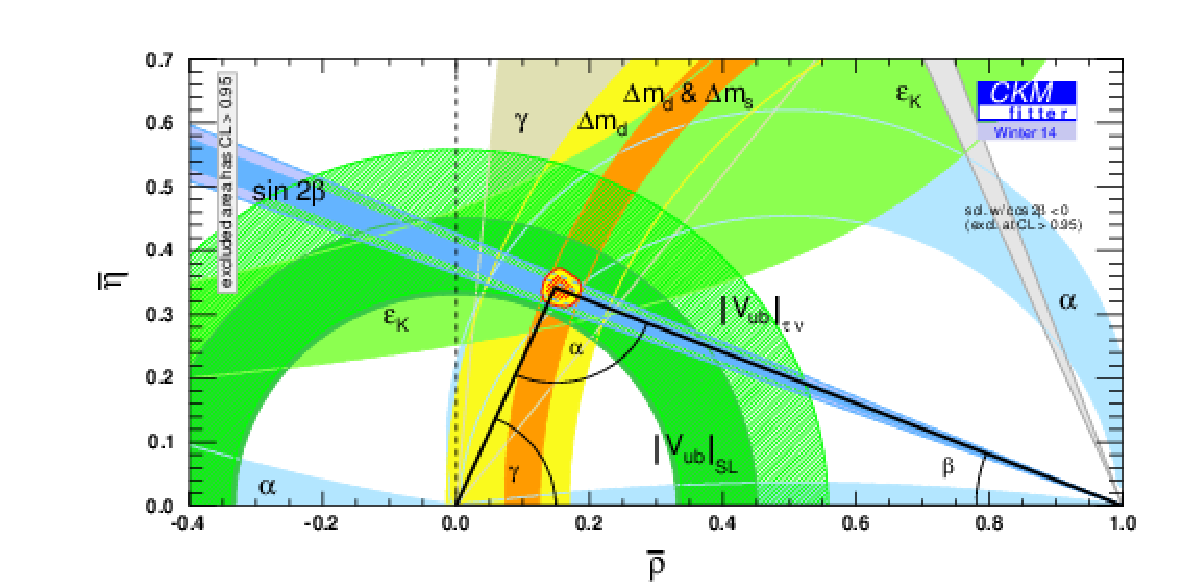
\includegraphics[width=0.5\textwidth]{rhoeta_small_Vub}
  %\end{center}
  %\caption[Unitary triangle measurements]{\small
    %Constraints on the UT in the complex plane. The $|\V{ub}|$ constraint is split into two
    %contributions: inclusive and exclusive semileptonic decays (plain dark green)
    %and $|\V{ub}|$ from \decay{\Bp}{\tau\nu_\tau} (hashed green).
    %The red hashed region of the global combination corresponds to 68\% CL.
  %}
  %\label{fig:th:ut2}
%\end{figure}

%\section{Testing the flavour sector of the SM}
%There are convincing/powerful/... reasons that

%If new physics were to enter as a CPV phase in the flavour sector of the SM, this would be seen in
%measurements of the angles and sides of the UT.
%The total particle physics Lagrangian can be written as:
%\begin{equation}
  %\Lag{Tot} = \Lag{SM} + \Lag{NP}.
%\end{equation}
%Additional CP-violating phases in \Lag{NP} would cause the triangle not to close, such that
%$\alpha+\beta+\gamma\neq\pi$.
%Therefore it is vital to measure the CKM matrix elements to as high a precision as possible in as
%many ways as possible.
%The current constraints on the UT are shown in Fig.~\ref{fig:th:ut2}.

%Diagonal elements of the CKM matrix are all known to high fractional precision...
